\documentclass[1p]{elsarticle_modified}
%\bibliographystyle{elsarticle-num}

%\usepackage[colorlinks]{hyperref}
%\usepackage{abbrmath_seonhwa} %\Abb, \Ascr, \Acal ,\Abf, \Afrak
\usepackage{amsfonts}
\usepackage{amssymb}
\usepackage{amsmath}
\usepackage{amsthm}
\usepackage{scalefnt}
\usepackage{amsbsy}
\usepackage{kotex}
\usepackage{caption}
\usepackage{subfig}
\usepackage{color}
\usepackage{graphicx}
\usepackage{xcolor} %% white, black, red, green, blue, cyan, magenta, yellow
\usepackage{float}
\usepackage{setspace}
\usepackage{hyperref}

\usepackage{tikz}
\usetikzlibrary{arrows}

\usepackage{multirow}
\usepackage{array} % fixed length table
\usepackage{hhline}

%%%%%%%%%%%%%%%%%%%%%
\makeatletter
\renewcommand*\env@matrix[1][\arraystretch]{%
	\edef\arraystretch{#1}%
	\hskip -\arraycolsep
	\let\@ifnextchar\new@ifnextchar
	\array{*\c@MaxMatrixCols c}}
\makeatother %https://tex.stackexchange.com/questions/14071/how-can-i-increase-the-line-spacing-in-a-matrix
%%%%%%%%%%%%%%%

\usepackage[normalem]{ulem}

\newcommand{\msout}[1]{\ifmmode\text{\sout{\ensuremath{#1}}}\else\sout{#1}\fi}
%SOURCE: \msout is \stkout macro in https://tex.stackexchange.com/questions/20609/strikeout-in-math-mode

\newcommand{\cancel}[1]{
	\ifmmode
	{\color{red}\msout{#1}}
	\else
	{\color{red}\sout{#1}}
	\fi
}

\newcommand{\add}[1]{
	{\color{blue}\uwave{#1}}
}

\newcommand{\replace}[2]{
	\ifmmode
	{\color{red}\msout{#1}}{\color{blue}\uwave{#2}}
	\else
	{\color{red}\sout{#1}}{\color{blue}\uwave{#2}}
	\fi
}

\newcommand{\Sol}{\mathcal{S}} %segment
\newcommand{\D}{D} %diagram
\newcommand{\A}{\mathcal{A}} %arc


%%%%%%%%%%%%%%%%%%%%%%%%%%%%%5 test

\def\sl{\operatorname{\textup{SL}}(2,\Cbb)}
\def\psl{\operatorname{\textup{PSL}}(2,\Cbb)}
\def\quan{\mkern 1mu \triangleright \mkern 1mu}

\theoremstyle{definition}
\newtheorem{thm}{Theorem}[section]
\newtheorem{prop}[thm]{Proposition}
\newtheorem{lem}[thm]{Lemma}
\newtheorem{ques}[thm]{Question}
\newtheorem{cor}[thm]{Corollary}
\newtheorem{defn}[thm]{Definition}
\newtheorem{exam}[thm]{Example}
\newtheorem{rmk}[thm]{Remark}
\newtheorem{alg}[thm]{Algorithm}

\newcommand{\I}{\sqrt{-1}}
\begin{document}

%\begin{frontmatter}
%
%\title{Boundary parabolic representations of knots up to 8 crossings}
%
%%% Group authors per affiliation:
%\author{Yunhi Cho} 
%\address{Department of Mathematics, University of Seoul, Seoul, Korea}
%\ead{yhcho@uos.ac.kr}
%
%
%\author{Seonhwa Kim} %\fnref{s_kim}}
%\address{Center for Geometry and Physics, Institute for Basic Science, Pohang, 37673, Korea}
%\ead{ryeona17@ibs.re.kr}
%
%\author{Hyuk Kim}
%\address{Department of Mathematical Sciences, Seoul National University, Seoul 08826, Korea}
%\ead{hyukkim@snu.ac.kr}
%
%\author{Seokbeom Yoon}
%\address{Department of Mathematical Sciences, Seoul National University, Seoul, 08826,  Korea}
%\ead{sbyoon15@snu.ac.kr}
%
%\begin{abstract}
%We find all boundary parabolic representation of knots up to 8 crossings.
%
%\end{abstract}
%\begin{keyword}
%    \MSC[2010] 57M25 
%\end{keyword}
%
%\end{frontmatter}

%\linenumbers
%\tableofcontents
%
\newcommand\colored[1]{\textcolor{white}{\rule[-0.35ex]{0.8em}{1.4ex}}\kern-0.8em\color{red} #1}%
%\newcommand\colored[1]{\textcolor{white}{ #1}\kern-2.17ex	\textcolor{white}{ #1}\kern-1.81ex	\textcolor{white}{ #1}\kern-2.15ex\color{red}#1	}

{\Large $\underline{12a_{1167}~(K12a_{1167})}$}

\setlength{\tabcolsep}{10pt}
\renewcommand{\arraystretch}{1.6}
\vspace{1cm}\begin{tabular}{m{100pt}>{\centering\arraybackslash}m{274pt}}
\multirow{5}{120pt}{
	\centering
	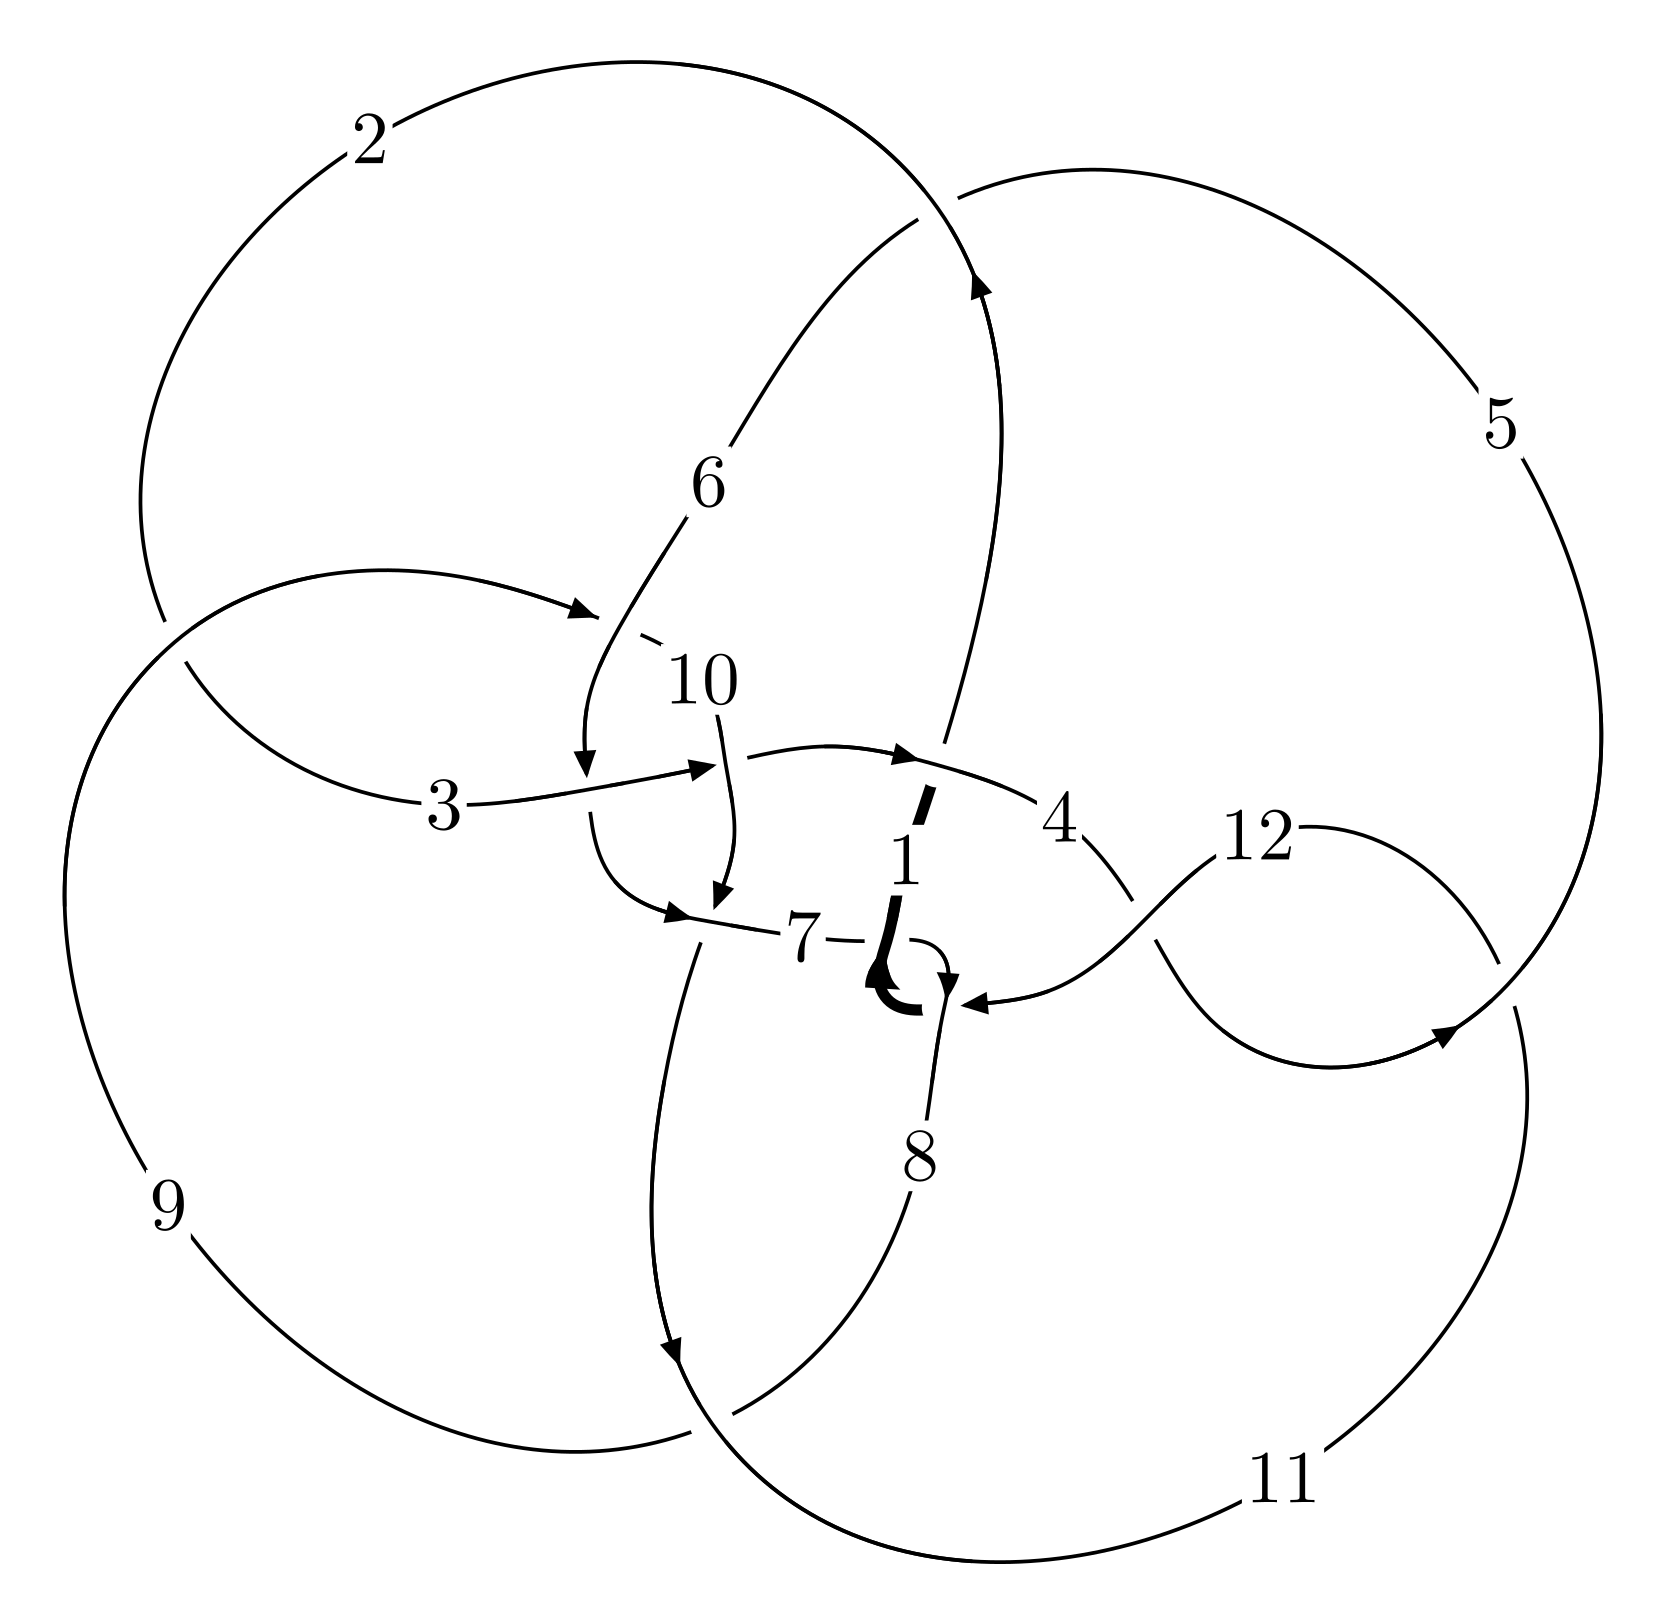
\includegraphics[width=112pt]{../../../GIT/diagram.site/Diagrams/png/1968_12a_1167.png}\\
\ \ \ A knot diagram\footnotemark}&
\allowdisplaybreaks
\textbf{Linearized knot diagam} \\
\cline{2-2}
 &
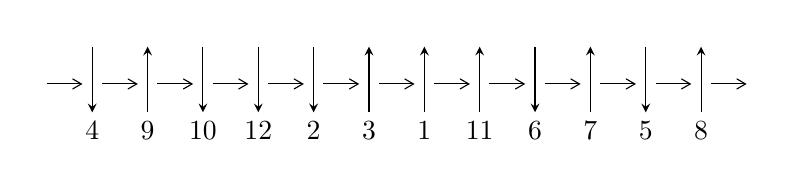
\begin{tikzpicture}[x=20pt, y=17pt]
	% nodes
	\node (C0) at (0, 0) {};
	\node (C1) at (1, 0) {};
	\node (C1U) at (1, +1) {};
	\node (C1D) at (1, -1) {4};

	\node (C2) at (2, 0) {};
	\node (C2U) at (2, +1) {};
	\node (C2D) at (2, -1) {9};

	\node (C3) at (3, 0) {};
	\node (C3U) at (3, +1) {};
	\node (C3D) at (3, -1) {10};

	\node (C4) at (4, 0) {};
	\node (C4U) at (4, +1) {};
	\node (C4D) at (4, -1) {12};

	\node (C5) at (5, 0) {};
	\node (C5U) at (5, +1) {};
	\node (C5D) at (5, -1) {2};

	\node (C6) at (6, 0) {};
	\node (C6U) at (6, +1) {};
	\node (C6D) at (6, -1) {3};

	\node (C7) at (7, 0) {};
	\node (C7U) at (7, +1) {};
	\node (C7D) at (7, -1) {1};

	\node (C8) at (8, 0) {};
	\node (C8U) at (8, +1) {};
	\node (C8D) at (8, -1) {11};

	\node (C9) at (9, 0) {};
	\node (C9U) at (9, +1) {};
	\node (C9D) at (9, -1) {6};

	\node (C10) at (10, 0) {};
	\node (C10U) at (10, +1) {};
	\node (C10D) at (10, -1) {7};

	\node (C11) at (11, 0) {};
	\node (C11U) at (11, +1) {};
	\node (C11D) at (11, -1) {5};

	\node (C12) at (12, 0) {};
	\node (C12U) at (12, +1) {};
	\node (C12D) at (12, -1) {8};
	\node (C13) at (13, 0) {};

	% arrows
	\draw[->,>={angle 60}]
	(C0) edge (C1) (C1) edge (C2) (C2) edge (C3) (C3) edge (C4) (C4) edge (C5) (C5) edge (C6) (C6) edge (C7) (C7) edge (C8) (C8) edge (C9) (C9) edge (C10) (C10) edge (C11) (C11) edge (C12) (C12) edge (C13) ;	\draw[->,>=stealth]
	(C1U) edge (C1D) (C2D) edge (C2U) (C3U) edge (C3D) (C4U) edge (C4D) (C5U) edge (C5D) (C6D) edge (C6U) (C7D) edge (C7U) (C8D) edge (C8U) (C9U) edge (C9D) (C10D) edge (C10U) (C11U) edge (C11D) (C12D) edge (C12U) ;
	\end{tikzpicture} \\
\hhline{~~} \\& 
\textbf{Solving Sequence} \\ \cline{2-2} 
 &
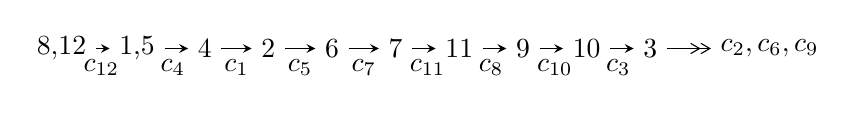
\begin{tikzpicture}[x=23pt, y=7pt]
	% node
	\node (A0) at (-1/8, 0) {8,12};
	\node (A1) at (17/16, 0) {1,5};
	\node (A2) at (17/8, 0) {4};
	\node (A3) at (25/8, 0) {2};
	\node (A4) at (33/8, 0) {6};
	\node (A5) at (41/8, 0) {7};
	\node (A6) at (49/8, 0) {11};
	\node (A7) at (57/8, 0) {9};
	\node (A8) at (65/8, 0) {10};
	\node (A9) at (73/8, 0) {3};
	\node (C1) at (1/2, -1) {$c_{12}$};
	\node (C2) at (13/8, -1) {$c_{4}$};
	\node (C3) at (21/8, -1) {$c_{1}$};
	\node (C4) at (29/8, -1) {$c_{5}$};
	\node (C5) at (37/8, -1) {$c_{7}$};
	\node (C6) at (45/8, -1) {$c_{11}$};
	\node (C7) at (53/8, -1) {$c_{8}$};
	\node (C8) at (61/8, -1) {$c_{10}$};
	\node (C9) at (69/8, -1) {$c_{3}$};
	\node (A10) at (11, 0) {$c_{2},c_{6},c_{9}$};

	% edge
	\draw[->,>=stealth]	
	(A0) edge (A1) (A1) edge (A2) (A2) edge (A3) (A3) edge (A4) (A4) edge (A5) (A5) edge (A6) (A6) edge (A7) (A7) edge (A8) (A8) edge (A9) ;
	\draw[->>,>={angle 60}]	
	(A9) edge (A10);
\end{tikzpicture} \\ 

\end{tabular} \\

\footnotetext{
The image of knot diagram is generated by the software ``\textbf{Draw programme}" developed by Andrew Bartholomew(\url{http://www.layer8.co.uk/maths/draw/index.htm\#Running-draw}), where we modified some parts for our purpose(\url{https://github.com/CATsTAILs/LinksPainter}).
}\phantom \\ \newline 
\centering \textbf{Ideals for irreducible components\footnotemark of $X_{\text{par}}$} 
 
\begin{align*}
I^u_{1}&=\langle 
4.59872\times10^{1554} u^{217}-9.84331\times10^{1554} u^{216}+\cdots+7.30909\times10^{1556} b-1.10702\times10^{1560},\\
\phantom{I^u_{1}}&\phantom{= \langle  }1.07881\times10^{1569} u^{217}+1.14742\times10^{1569} u^{216}+\cdots+8.66519\times10^{1570} a+2.46881\times10^{1575},\\
\phantom{I^u_{1}}&\phantom{= \langle  }u^{218}- u^{217}+\cdots+1084332 u+800958\rangle \\
I^u_{2}&=\langle 
8.39999\times10^{88} u^{59}-2.76464\times10^{88} u^{58}+\cdots+8.73404\times10^{87} b-3.20535\times10^{89},\\
\phantom{I^u_{2}}&\phantom{= \langle  }-6.26274\times10^{91} u^{59}-5.42884\times10^{91} u^{58}+\cdots+1.55466\times10^{91} a-9.36581\times10^{92},\\
\phantom{I^u_{2}}&\phantom{= \langle  }u^{60}+21 u^{58}+\cdots+40 u+20\rangle \\
\\
\end{align*}
\raggedright * 2 irreducible components of $\dim_{\mathbb{C}}=0$, with total 278 representations.\\
\footnotetext{All coefficients of polynomials are rational numbers. But the coefficients are sometimes approximated in decimal forms when there is not enough margin.}
\newpage
\renewcommand{\arraystretch}{1}
\centering \section*{I. $I^u_{1}= \langle 4.60\times10^{1554} u^{217}-9.84\times10^{1554} u^{216}+\cdots+7.31\times10^{1556} b-1.11\times10^{1560},\;1.08\times10^{1569} u^{217}+1.15\times10^{1569} u^{216}+\cdots+8.67\times10^{1570} a+2.47\times10^{1575},\;u^{218}- u^{217}+\cdots+1084332 u+800958 \rangle$}
\flushleft \textbf{(i) Arc colorings}\\
\begin{tabular}{m{7pt} m{180pt} m{7pt} m{180pt} }
\flushright $a_{8}=$&$\begin{pmatrix}0\\u\end{pmatrix}$ \\
\flushright $a_{12}=$&$\begin{pmatrix}1\\0\end{pmatrix}$ \\
\flushright $a_{1}=$&$\begin{pmatrix}1\\- u^2\end{pmatrix}$ \\
\flushright $a_{5}=$&$\begin{pmatrix}-0.0124500 u^{217}-0.0132417 u^{216}+\cdots-57143.3 u-28491.1\\-0.00629178 u^{217}+0.0134672 u^{216}+\cdots-5937.11 u+1514.57\end{pmatrix}$ \\
\flushright $a_{4}=$&$\begin{pmatrix}-0.0187418 u^{217}+0.000225544 u^{216}+\cdots-63080.4 u-26976.6\\-0.00629178 u^{217}+0.0134672 u^{216}+\cdots-5937.11 u+1514.57\end{pmatrix}$ \\
\flushright $a_{2}=$&$\begin{pmatrix}-0.0200316 u^{217}+0.0391073 u^{216}+\cdots+40964.8 u+19242.7\\-0.0144419 u^{217}+0.0238159 u^{216}+\cdots-25081.4 u+1435.38\end{pmatrix}$ \\
\flushright $a_{6}=$&$\begin{pmatrix}0.0378271 u^{217}-0.0347035 u^{216}+\cdots+77782.1 u+773.143\\-0.00425950 u^{217}+0.0280317 u^{216}+\cdots+14309.1 u+20325.0\end{pmatrix}$ \\
\flushright $a_{7}=$&$\begin{pmatrix}- u\\u^3+u\end{pmatrix}$ \\
\flushright $a_{11}=$&$\begin{pmatrix}-0.0210500 u^{217}+0.0336813 u^{216}+\cdots-24851.7 u+3718.28\\0.0149998 u^{217}-0.0269724 u^{216}+\cdots+20949.7 u-907.805\end{pmatrix}$ \\
\flushright $a_{9}=$&$\begin{pmatrix}0.00566707 u^{217}+0.0502761 u^{216}+\cdots+49142.3 u+27148.3\\0.0461777 u^{217}-0.0612084 u^{216}+\cdots+61781.7 u+17922.2\end{pmatrix}$ \\
\flushright $a_{10}=$&$\begin{pmatrix}-0.0296511 u^{217}+0.0393404 u^{216}+\cdots-37179.5 u-3303.97\\0.0174703 u^{217}-0.0258301 u^{216}+\cdots+23198.2 u+3757.99\end{pmatrix}$ \\
\flushright $a_{3}=$&$\begin{pmatrix}-0.0266976 u^{217}-0.0219209 u^{216}+\cdots-69036.9 u-44256.4\\-0.0194184 u^{217}+0.0258173 u^{216}+\cdots-36011.2 u-10545.3\end{pmatrix}$\\&\end{tabular}
\flushleft \textbf{(ii) Obstruction class $= -1$}\\~\\
\flushleft \textbf{(iii) Cusp Shapes $= -0.102226 u^{217}+0.313054 u^{216}+\cdots+38230.4 u+152101.$}\\~\\
\newpage\renewcommand{\arraystretch}{1}
\flushleft \textbf{(iv) u-Polynomials at the component}\newline \\
\begin{tabular}{m{50pt}|m{274pt}}
Crossings & \hspace{64pt}u-Polynomials at each crossing \\
\hline $$\begin{aligned}c_{1}\end{aligned}$$&$\begin{aligned}
&u^{218}+7 u^{217}+\cdots-325966059 u+13035439
\end{aligned}$\\
\hline $$\begin{aligned}c_{2}\end{aligned}$$&$\begin{aligned}
&6(6 u^{218}-6 u^{217}+\cdots-603 u+1721)
\end{aligned}$\\
\hline $$\begin{aligned}c_{3}\end{aligned}$$&$\begin{aligned}
&6(6 u^{218}+6 u^{217}+\cdots+603 u+1721)
\end{aligned}$\\
\hline $$\begin{aligned}c_{4},c_{11}\end{aligned}$$&$\begin{aligned}
&u^{218}+u^{217}+\cdots-1084332 u+800958
\end{aligned}$\\
\hline $$\begin{aligned}c_{5}\end{aligned}$$&$\begin{aligned}
&u^{218}-6 u^{217}+\cdots-4497810 u+159275
\end{aligned}$\\
\hline $$\begin{aligned}c_{6}\end{aligned}$$&$\begin{aligned}
&u^{218}-7 u^{217}+\cdots+5706 u+1086
\end{aligned}$\\
\hline $$\begin{aligned}c_{7},c_{12}\end{aligned}$$&$\begin{aligned}
&u^{218}- u^{217}+\cdots+1084332 u+800958
\end{aligned}$\\
\hline $$\begin{aligned}c_{8}\end{aligned}$$&$\begin{aligned}
&u^{218}-7 u^{217}+\cdots+325966059 u+13035439
\end{aligned}$\\
\hline $$\begin{aligned}c_{9}\end{aligned}$$&$\begin{aligned}
&u^{218}+7 u^{217}+\cdots-5706 u+1086
\end{aligned}$\\
\hline $$\begin{aligned}c_{10}\end{aligned}$$&$\begin{aligned}
&u^{218}+6 u^{217}+\cdots+4497810 u+159275
\end{aligned}$\\
\hline
\end{tabular}\\~\\
\newpage\renewcommand{\arraystretch}{1}
\flushleft \textbf{(v) Riley Polynomials at the component}\newline \\
\begin{tabular}{m{50pt}|m{274pt}}
Crossings & \hspace{64pt}Riley Polynomials at each crossing \\
\hline $$\begin{aligned}c_{1},c_{8}\end{aligned}$$&$\begin{aligned}
&y^{218}-27 y^{217}+\cdots-75149030070299023 y+169922669922721
\end{aligned}$\\
\hline $$\begin{aligned}c_{2},c_{3}\end{aligned}$$&$\begin{aligned}
&36(36 y^{218}+228 y^{217}+\cdots-2.18635\times10^{8} y+2961841)
\end{aligned}$\\
\hline $$\begin{aligned}c_{4},c_{7},c_{11}\\c_{12}\end{aligned}$$&$\begin{aligned}
&y^{218}+127 y^{217}+\cdots+37988843650536 y+641533717764
\end{aligned}$\\
\hline $$\begin{aligned}c_{5},c_{10}\end{aligned}$$&$\begin{aligned}
&y^{218}-26 y^{217}+\cdots-2357094900150 y+25368525625
\end{aligned}$\\
\hline $$\begin{aligned}c_{6},c_{9}\end{aligned}$$&$\begin{aligned}
&y^{218}-7 y^{217}+\cdots-16168524 y+1179396
\end{aligned}$\\
\hline
\end{tabular}\\~\\
\newpage\flushleft \textbf{(vi) Complex Volumes and Cusp Shapes}
$$\begin{array}{c|c|c}  
\text{Solutions to }I^u_{1}& \I (\text{vol} + \sqrt{-1}CS) & \text{Cusp shape}\\
 \hline 
\begin{aligned}
u &= -0.437041 + 0.900025 I \\
a &= -0.212197 + 0.783889 I \\
b &= \phantom{-}0.470183 - 1.256570 I\end{aligned}
 & \phantom{-}1.89033 + 0.72271 I & \phantom{-0.000000 } 0 \\ \hline\begin{aligned}
u &= -0.437041 - 0.900025 I \\
a &= -0.212197 - 0.783889 I \\
b &= \phantom{-}0.470183 + 1.256570 I\end{aligned}
 & \phantom{-}1.89033 - 0.72271 I & \phantom{-0.000000 } 0 \\ \hline\begin{aligned}
u &= -1.003990 + 0.150540 I \\
a &= \phantom{-}0.46765 + 1.53202 I \\
b &= -0.394463 - 1.163640 I\end{aligned}
 & \phantom{-}1.04005 - 7.54869 I & \phantom{-0.000000 } 0 \\ \hline\begin{aligned}
u &= -1.003990 - 0.150540 I \\
a &= \phantom{-}0.46765 - 1.53202 I \\
b &= -0.394463 + 1.163640 I\end{aligned}
 & \phantom{-}1.04005 + 7.54869 I & \phantom{-0.000000 } 0 \\ \hline\begin{aligned}
u &= -0.100843 + 0.975368 I \\
a &= \phantom{-}0.608586 + 0.384135 I \\
b &= -0.462739 + 0.668047 I\end{aligned}
 & -2.24226 + 5.02667 I & \phantom{-0.000000 } 0 \\ \hline\begin{aligned}
u &= -0.100843 - 0.975368 I \\
a &= \phantom{-}0.608586 - 0.384135 I \\
b &= -0.462739 - 0.668047 I\end{aligned}
 & -2.24226 - 5.02667 I & \phantom{-0.000000 } 0 \\ \hline\begin{aligned}
u &= \phantom{-}0.308123 + 0.973343 I \\
a &= \phantom{-}0.052320 + 0.205725 I \\
b &= \phantom{-}1.035720 - 0.074637 I\end{aligned}
 & -1.48317 + 2.08145 I & \phantom{-0.000000 } 0 \\ \hline\begin{aligned}
u &= \phantom{-}0.308123 - 0.973343 I \\
a &= \phantom{-}0.052320 - 0.205725 I \\
b &= \phantom{-}1.035720 + 0.074637 I\end{aligned}
 & -1.48317 - 2.08145 I & \phantom{-0.000000 } 0 \\ \hline\begin{aligned}
u &= -0.613126 + 0.759553 I \\
a &= \phantom{-}1.40770 - 0.75603 I \\
b &= \phantom{-}0.499855 + 0.732282 I\end{aligned}
 & \phantom{-}1.94446 + 0.55451 I & \phantom{-0.000000 } 0 \\ \hline\begin{aligned}
u &= -0.613126 - 0.759553 I \\
a &= \phantom{-}1.40770 + 0.75603 I \\
b &= \phantom{-}0.499855 - 0.732282 I\end{aligned}
 & \phantom{-}1.94446 - 0.55451 I & \phantom{-0.000000 } 0\\
 \hline 
 \end{array}$$\newpage$$\begin{array}{c|c|c}  
\text{Solutions to }I^u_{1}& \I (\text{vol} + \sqrt{-1}CS) & \text{Cusp shape}\\
 \hline 
\begin{aligned}
u &= -0.462881 + 0.921010 I \\
a &= \phantom{-}1.65931 - 0.95682 I \\
b &= \phantom{-}0.303325 + 1.215080 I\end{aligned}
 & \phantom{-}5.39866 - 2.44724 I & \phantom{-0.000000 } 0 \\ \hline\begin{aligned}
u &= -0.462881 - 0.921010 I \\
a &= \phantom{-}1.65931 + 0.95682 I \\
b &= \phantom{-}0.303325 - 1.215080 I\end{aligned}
 & \phantom{-}5.39866 + 2.44724 I & \phantom{-0.000000 } 0 \\ \hline\begin{aligned}
u &= \phantom{-}1.035720 + 0.074637 I \\
a &= -0.123358 + 1.070400 I \\
b &= \phantom{-}0.308123 - 0.973343 I\end{aligned}
 & \phantom{-}1.48317 + 2.08145 I & \phantom{-0.000000 } 0 \\ \hline\begin{aligned}
u &= \phantom{-}1.035720 - 0.074637 I \\
a &= -0.123358 - 1.070400 I \\
b &= \phantom{-}0.308123 + 0.973343 I\end{aligned}
 & \phantom{-}1.48317 - 2.08145 I & \phantom{-0.000000 } 0 \\ \hline\begin{aligned}
u &= -1.019800 + 0.230367 I \\
a &= \phantom{-}0.04271 - 1.76667 I \\
b &= -0.245349 + 1.164410 I\end{aligned}
 & \phantom{-}5.69009 + 2.69649 I & \phantom{-0.000000 } 0 \\ \hline\begin{aligned}
u &= -1.019800 - 0.230367 I \\
a &= \phantom{-}0.04271 + 1.76667 I \\
b &= -0.245349 - 1.164410 I\end{aligned}
 & \phantom{-}5.69009 - 2.69649 I & \phantom{-0.000000 } 0 \\ \hline\begin{aligned}
u &= -0.940943 + 0.473748 I \\
a &= -0.511895 + 1.294760 I \\
b &= \phantom{-}0.551520 - 1.222040 I\end{aligned}
 & \phantom{-}3.67220 + 6.74825 I & \phantom{-0.000000 } 0 \\ \hline\begin{aligned}
u &= -0.940943 - 0.473748 I \\
a &= -0.511895 - 1.294760 I \\
b &= \phantom{-}0.551520 + 1.222040 I\end{aligned}
 & \phantom{-}3.67220 - 6.74825 I & \phantom{-0.000000 } 0 \\ \hline\begin{aligned}
u &= \phantom{-}0.417538 + 0.847320 I \\
a &= -0.434386 - 1.022500 I \\
b &= \phantom{-}0.14556 + 1.62539 I\end{aligned}
 & \phantom{-}3.61073 + 9.93097 I & \phantom{-0.000000 } 0 \\ \hline\begin{aligned}
u &= \phantom{-}0.417538 - 0.847320 I \\
a &= -0.434386 + 1.022500 I \\
b &= \phantom{-}0.14556 - 1.62539 I\end{aligned}
 & \phantom{-}3.61073 - 9.93097 I & \phantom{-0.000000 } 0\\
 \hline 
 \end{array}$$\newpage$$\begin{array}{c|c|c}  
\text{Solutions to }I^u_{1}& \I (\text{vol} + \sqrt{-1}CS) & \text{Cusp shape}\\
 \hline 
\begin{aligned}
u &= \phantom{-}0.918583 + 0.207533 I \\
a &= \phantom{-}0.158984 + 1.222530 I \\
b &= \phantom{-}0.617526 - 0.420082 I\end{aligned}
 & -0.55926 - 1.41093 I & \phantom{-0.000000 } 0 \\ \hline\begin{aligned}
u &= \phantom{-}0.918583 - 0.207533 I \\
a &= \phantom{-}0.158984 - 1.222530 I \\
b &= \phantom{-}0.617526 + 0.420082 I\end{aligned}
 & -0.55926 + 1.41093 I & \phantom{-0.000000 } 0 \\ \hline\begin{aligned}
u &= -0.876472 + 0.598057 I \\
a &= \phantom{-}0.85061 - 1.35338 I \\
b &= -0.212076 + 1.158300 I\end{aligned}
 & \phantom{-}4.47322 + 1.53890 I & \phantom{-0.000000 } 0 \\ \hline\begin{aligned}
u &= -0.876472 - 0.598057 I \\
a &= \phantom{-}0.85061 + 1.35338 I \\
b &= -0.212076 - 1.158300 I\end{aligned}
 & \phantom{-}4.47322 - 1.53890 I & \phantom{-0.000000 } 0 \\ \hline\begin{aligned}
u &= \phantom{-}0.280150 + 1.026020 I \\
a &= \phantom{-}2.78942 + 0.08607 I \\
b &= \phantom{-}0.222875 - 1.137530 I\end{aligned}
 & \phantom{-}1.77355 + 9.93813 I & \phantom{-0.000000 } 0 \\ \hline\begin{aligned}
u &= \phantom{-}0.280150 - 1.026020 I \\
a &= \phantom{-}2.78942 - 0.08607 I \\
b &= \phantom{-}0.222875 + 1.137530 I\end{aligned}
 & \phantom{-}1.77355 - 9.93813 I & \phantom{-0.000000 } 0 \\ \hline\begin{aligned}
u &= -0.305306 + 0.885243 I \\
a &= -1.67577 + 0.37643 I \\
b &= -0.441025 - 1.259580 I\end{aligned}
 & \phantom{-}4.46515 - 1.74939 I & \phantom{-0.000000 } 0 \\ \hline\begin{aligned}
u &= -0.305306 - 0.885243 I \\
a &= -1.67577 - 0.37643 I \\
b &= -0.441025 + 1.259580 I\end{aligned}
 & \phantom{-}4.46515 + 1.74939 I & \phantom{-0.000000 } 0 \\ \hline\begin{aligned}
u &= -0.683089 + 0.622922 I \\
a &= -1.30428 + 2.09014 I \\
b &= \phantom{-}0.169104 - 0.739046 I\end{aligned}
 & \phantom{-}0.471008 + 0.398019 I & \phantom{-0.000000 } 0 \\ \hline\begin{aligned}
u &= -0.683089 - 0.622922 I \\
a &= -1.30428 - 2.09014 I \\
b &= \phantom{-}0.169104 + 0.739046 I\end{aligned}
 & \phantom{-}0.471008 - 0.398019 I & \phantom{-0.000000 } 0\\
 \hline 
 \end{array}$$\newpage$$\begin{array}{c|c|c}  
\text{Solutions to }I^u_{1}& \I (\text{vol} + \sqrt{-1}CS) & \text{Cusp shape}\\
 \hline 
\begin{aligned}
u &= \phantom{-}0.599761 + 0.900295 I \\
a &= \phantom{-}0.936810 + 0.857137 I \\
b &= \phantom{-}0.535570 - 1.197750 I\end{aligned}
 & \phantom{-}1.59135 + 1.88450 I & \phantom{-0.000000 } 0 \\ \hline\begin{aligned}
u &= \phantom{-}0.599761 - 0.900295 I \\
a &= \phantom{-}0.936810 - 0.857137 I \\
b &= \phantom{-}0.535570 + 1.197750 I\end{aligned}
 & \phantom{-}1.59135 - 1.88450 I & \phantom{-0.000000 } 0 \\ \hline\begin{aligned}
u &= \phantom{-}0.654387 + 0.863274 I \\
a &= -1.18552 - 0.97649 I \\
b &= -0.712791 + 1.018320 I\end{aligned}
 & \phantom{-}3.35203 + 9.91892 I & \phantom{-0.000000 } 0 \\ \hline\begin{aligned}
u &= \phantom{-}0.654387 - 0.863274 I \\
a &= -1.18552 + 0.97649 I \\
b &= -0.712791 - 1.018320 I\end{aligned}
 & \phantom{-}3.35203 - 9.91892 I & \phantom{-0.000000 } 0 \\ \hline\begin{aligned}
u &= \phantom{-}0.852196 + 0.669721 I \\
a &= -0.078282 - 0.811383 I \\
b &= \phantom{-}0.465569 + 1.148550 I\end{aligned}
 & \phantom{-}3.96693 - 4.42004 I & \phantom{-0.000000 } 0 \\ \hline\begin{aligned}
u &= \phantom{-}0.852196 - 0.669721 I \\
a &= -0.078282 + 0.811383 I \\
b &= \phantom{-}0.465569 - 1.148550 I\end{aligned}
 & \phantom{-}3.96693 + 4.42004 I & \phantom{-0.000000 } 0 \\ \hline\begin{aligned}
u &= -0.297555 + 0.858019 I \\
a &= -1.63283 + 1.32850 I \\
b &= -0.11319 - 1.61653 I\end{aligned}
 & \phantom{-}5.12076 - 1.34522 I & \phantom{-0.000000 } 0 \\ \hline\begin{aligned}
u &= -0.297555 - 0.858019 I \\
a &= -1.63283 - 1.32850 I \\
b &= -0.11319 + 1.61653 I\end{aligned}
 & \phantom{-}5.12076 + 1.34522 I & \phantom{-0.000000 } 0 \\ \hline\begin{aligned}
u &= \phantom{-}0.048733 + 0.898701 I \\
a &= -0.637885 + 0.115788 I \\
b &= -1.56815 - 0.17899 I\end{aligned}
 & -5.09439 - 4.03171 I & \phantom{-0.000000 } 0 \\ \hline\begin{aligned}
u &= \phantom{-}0.048733 - 0.898701 I \\
a &= -0.637885 - 0.115788 I \\
b &= -1.56815 + 0.17899 I\end{aligned}
 & -5.09439 + 4.03171 I & \phantom{-0.000000 } 0\\
 \hline 
 \end{array}$$\newpage$$\begin{array}{c|c|c}  
\text{Solutions to }I^u_{1}& \I (\text{vol} + \sqrt{-1}CS) & \text{Cusp shape}\\
 \hline 
\begin{aligned}
u &= \phantom{-}0.231329 + 1.076970 I \\
a &= \phantom{-}0.210849 + 0.060273 I \\
b &= \phantom{-}1.45238 + 0.43315 I\end{aligned}
 & -6.24818 + 5.10916 I & \phantom{-0.000000 } 0 \\ \hline\begin{aligned}
u &= \phantom{-}0.231329 - 1.076970 I \\
a &= \phantom{-}0.210849 - 0.060273 I \\
b &= \phantom{-}1.45238 - 0.43315 I\end{aligned}
 & -6.24818 - 5.10916 I & \phantom{-0.000000 } 0 \\ \hline\begin{aligned}
u &= -0.231325 + 1.078200 I \\
a &= \phantom{-}0.154807 - 0.301137 I \\
b &= \phantom{-}1.31711 - 0.51509 I\end{aligned}
 & -6.50971 + 3.37301 I & \phantom{-0.000000 } 0 \\ \hline\begin{aligned}
u &= -0.231325 - 1.078200 I \\
a &= \phantom{-}0.154807 + 0.301137 I \\
b &= \phantom{-}1.31711 + 0.51509 I\end{aligned}
 & -6.50971 - 3.37301 I & \phantom{-0.000000 } 0 \\ \hline\begin{aligned}
u &= \phantom{-}0.457581 + 1.005390 I \\
a &= \phantom{-}0.838236 + 0.551028 I \\
b &= \phantom{-}0.80753 - 1.19940 I\end{aligned}
 & \phantom{-}2.18813 + 2.01931 I & \phantom{-0.000000 } 0 \\ \hline\begin{aligned}
u &= \phantom{-}0.457581 - 1.005390 I \\
a &= \phantom{-}0.838236 - 0.551028 I \\
b &= \phantom{-}0.80753 + 1.19940 I\end{aligned}
 & \phantom{-}2.18813 - 2.01931 I & \phantom{-0.000000 } 0 \\ \hline\begin{aligned}
u &= -0.456995 + 1.006320 I \\
a &= \phantom{-}0.461164 - 0.001249 I \\
b &= \phantom{-}0.659626 - 0.133765 I\end{aligned}
 & \phantom{-}0.871914 + 0.606568 I & \phantom{-0.000000 } 0 \\ \hline\begin{aligned}
u &= -0.456995 - 1.006320 I \\
a &= \phantom{-}0.461164 + 0.001249 I \\
b &= \phantom{-}0.659626 + 0.133765 I\end{aligned}
 & \phantom{-}0.871914 - 0.606568 I & \phantom{-0.000000 } 0 \\ \hline\begin{aligned}
u &= \phantom{-}0.587380 + 0.938448 I \\
a &= \phantom{-}0.904126 + 0.520229 I \\
b &= -0.141926 - 0.323075 I\end{aligned}
 & -1.79288 + 4.49429 I & \phantom{-0.000000 } 0 \\ \hline\begin{aligned}
u &= \phantom{-}0.587380 - 0.938448 I \\
a &= \phantom{-}0.904126 - 0.520229 I \\
b &= -0.141926 + 0.323075 I\end{aligned}
 & -1.79288 - 4.49429 I & \phantom{-0.000000 } 0\\
 \hline 
 \end{array}$$\newpage$$\begin{array}{c|c|c}  
\text{Solutions to }I^u_{1}& \I (\text{vol} + \sqrt{-1}CS) & \text{Cusp shape}\\
 \hline 
\begin{aligned}
u &= \phantom{-}0.001784 + 0.890176 I \\
a &= \phantom{-}1.47851 - 1.97142 I \\
b &= \phantom{-}0.414190 + 1.163180 I\end{aligned}
 & -1.49293 - 5.19189 I & \phantom{-0.000000 } 0 \\ \hline\begin{aligned}
u &= \phantom{-}0.001784 - 0.890176 I \\
a &= \phantom{-}1.47851 + 1.97142 I \\
b &= \phantom{-}0.414190 - 1.163180 I\end{aligned}
 & -1.49293 + 5.19189 I & \phantom{-0.000000 } 0 \\ \hline\begin{aligned}
u &= \phantom{-}0.499855 + 0.732282 I \\
a &= -0.63104 - 2.00328 I \\
b &= -0.613126 + 0.759553 I\end{aligned}
 & -1.94446 - 0.55451 I & \phantom{-0.000000 } 0 \\ \hline\begin{aligned}
u &= \phantom{-}0.499855 - 0.732282 I \\
a &= -0.63104 + 2.00328 I \\
b &= -0.613126 - 0.759553 I\end{aligned}
 & -1.94446 + 0.55451 I & \phantom{-0.000000 } 0 \\ \hline\begin{aligned}
u &= -0.400012 + 0.781762 I \\
a &= \phantom{-}1.55396 - 2.03173 I \\
b &= \phantom{-}0.02640 + 1.45390 I\end{aligned}
 & \phantom{-}6.08780 - 1.75437 I & \phantom{-0.000000 } 0 \\ \hline\begin{aligned}
u &= -0.400012 - 0.781762 I \\
a &= \phantom{-}1.55396 + 2.03173 I \\
b &= \phantom{-}0.02640 - 1.45390 I\end{aligned}
 & \phantom{-}6.08780 + 1.75437 I & \phantom{-0.000000 } 0 \\ \hline\begin{aligned}
u &= -0.249759 + 0.838626 I \\
a &= -0.50515 + 1.32541 I \\
b &= \phantom{-}0.17906 - 1.59970 I\end{aligned}
 & \phantom{-}4.72681 - 0.80347 I & \phantom{-0.000000 } 0 \\ \hline\begin{aligned}
u &= -0.249759 - 0.838626 I \\
a &= -0.50515 - 1.32541 I \\
b &= \phantom{-}0.17906 + 1.59970 I\end{aligned}
 & \phantom{-}4.72681 + 0.80347 I & \phantom{-0.000000 } 0 \\ \hline\begin{aligned}
u &= -0.347244 + 0.800650 I \\
a &= \phantom{-}0.06808 - 2.15938 I \\
b &= \phantom{-}0.146770 + 1.255100 I\end{aligned}
 & \phantom{-}2.93174 - 5.03893 I & \phantom{-0.000000 } 0 \\ \hline\begin{aligned}
u &= -0.347244 - 0.800650 I \\
a &= \phantom{-}0.06808 + 2.15938 I \\
b &= \phantom{-}0.146770 - 1.255100 I\end{aligned}
 & \phantom{-}2.93174 + 5.03893 I & \phantom{-0.000000 } 0\\
 \hline 
 \end{array}$$\newpage$$\begin{array}{c|c|c}  
\text{Solutions to }I^u_{1}& \I (\text{vol} + \sqrt{-1}CS) & \text{Cusp shape}\\
 \hline 
\begin{aligned}
u &= -0.360891 + 0.783303 I \\
a &= \phantom{-}2.43073 - 0.59779 I \\
b &= -0.028929 + 0.843147 I\end{aligned}
 & \phantom{-}2.95474 + 1.76216 I & \phantom{-0.000000 } 0 \\ \hline\begin{aligned}
u &= -0.360891 - 0.783303 I \\
a &= \phantom{-}2.43073 + 0.59779 I \\
b &= -0.028929 - 0.843147 I\end{aligned}
 & \phantom{-}2.95474 - 1.76216 I & \phantom{-0.000000 } 0 \\ \hline\begin{aligned}
u &= \phantom{-}0.478952 + 0.712106 I \\
a &= -1.53516 - 0.79069 I \\
b &= -0.423654 + 1.290220 I\end{aligned}
 & \phantom{-}3.95917 - 6.15252 I & \phantom{-0.000000 } 0 \\ \hline\begin{aligned}
u &= \phantom{-}0.478952 - 0.712106 I \\
a &= -1.53516 + 0.79069 I \\
b &= -0.423654 - 1.290220 I\end{aligned}
 & \phantom{-}3.95917 + 6.15252 I & \phantom{-0.000000 } 0 \\ \hline\begin{aligned}
u &= -0.028929 + 0.843147 I \\
a &= -2.16685 - 1.18164 I \\
b &= -0.360891 + 0.783303 I\end{aligned}
 & -2.95474 - 1.76216 I & \phantom{-0.000000 } 0 \\ \hline\begin{aligned}
u &= -0.028929 - 0.843147 I \\
a &= -2.16685 + 1.18164 I \\
b &= -0.360891 - 0.783303 I\end{aligned}
 & -2.95474 + 1.76216 I & \phantom{-0.000000 } 0 \\ \hline\begin{aligned}
u &= \phantom{-}0.222875 + 1.137530 I \\
a &= \phantom{-}2.04824 + 2.09156 I \\
b &= \phantom{-}0.280150 - 1.026020 I\end{aligned}
 & -1.77355 + 9.93813 I & \phantom{-0.000000 } 0 \\ \hline\begin{aligned}
u &= \phantom{-}0.222875 - 1.137530 I \\
a &= \phantom{-}2.04824 - 2.09156 I \\
b &= \phantom{-}0.280150 + 1.026020 I\end{aligned}
 & -1.77355 - 9.93813 I & \phantom{-0.000000 } 0 \\ \hline\begin{aligned}
u &= \phantom{-}0.492848 + 1.054720 I \\
a &= \phantom{-}0.066722 - 0.384063 I \\
b &= -1.204180 - 0.427493 I\end{aligned}
 & -1.31280 + 5.76610 I & \phantom{-0.000000 } 0 \\ \hline\begin{aligned}
u &= \phantom{-}0.492848 - 1.054720 I \\
a &= \phantom{-}0.066722 + 0.384063 I \\
b &= -1.204180 + 0.427493 I\end{aligned}
 & -1.31280 - 5.76610 I & \phantom{-0.000000 } 0\\
 \hline 
 \end{array}$$\newpage$$\begin{array}{c|c|c}  
\text{Solutions to }I^u_{1}& \I (\text{vol} + \sqrt{-1}CS) & \text{Cusp shape}\\
 \hline 
\begin{aligned}
u &= -0.485058 + 0.675673 I \\
a &= \phantom{-}0.71648 - 1.71839 I \\
b &= -0.09723 + 1.42923 I\end{aligned}
 & \phantom{-}6.16346 - 1.48072 I & \phantom{-0.000000 } 0 \\ \hline\begin{aligned}
u &= -0.485058 - 0.675673 I \\
a &= \phantom{-}0.71648 + 1.71839 I \\
b &= -0.09723 - 1.42923 I\end{aligned}
 & \phantom{-}6.16346 + 1.48072 I & \phantom{-0.000000 } 0 \\ \hline\begin{aligned}
u &= -0.334184 + 1.120090 I \\
a &= -1.087770 + 0.371028 I \\
b &= -0.778130 - 1.146260 I\end{aligned}
 & \phantom{-}0.68932 - 6.27683 I & \phantom{-0.000000 } 0 \\ \hline\begin{aligned}
u &= -0.334184 - 1.120090 I \\
a &= -1.087770 - 0.371028 I \\
b &= -0.778130 + 1.146260 I\end{aligned}
 & \phantom{-}0.68932 + 6.27683 I & \phantom{-0.000000 } 0 \\ \hline\begin{aligned}
u &= -1.128100 + 0.310890 I \\
a &= \phantom{-}0.44682 - 1.47507 I \\
b &= -0.474782 + 1.184610 I\end{aligned}
 & \phantom{-}4.45442 + 7.05483 I & \phantom{-0.000000 } 0 \\ \hline\begin{aligned}
u &= -1.128100 - 0.310890 I \\
a &= \phantom{-}0.44682 + 1.47507 I \\
b &= -0.474782 - 1.184610 I\end{aligned}
 & \phantom{-}4.45442 - 7.05483 I & \phantom{-0.000000 } 0 \\ \hline\begin{aligned}
u &= -0.212076 + 1.158300 I \\
a &= -0.529572 - 0.285491 I \\
b &= -0.876472 + 0.598057 I\end{aligned}
 & -4.47322 - 1.53890 I & \phantom{-0.000000 } 0 \\ \hline\begin{aligned}
u &= -0.212076 - 1.158300 I \\
a &= -0.529572 + 0.285491 I \\
b &= -0.876472 - 0.598057 I\end{aligned}
 & -4.47322 + 1.53890 I & \phantom{-0.000000 } 0 \\ \hline\begin{aligned}
u &= -0.815024 + 0.089394 I \\
a &= \phantom{-}0.298810 + 1.035750 I \\
b &= -0.815024 - 0.089394 I\end{aligned}
 & \phantom{-0.000000 -}10.6392 I & \phantom{-0.000000 } 0 \\ \hline\begin{aligned}
u &= -0.815024 - 0.089394 I \\
a &= \phantom{-}0.298810 - 1.035750 I \\
b &= -0.815024 + 0.089394 I\end{aligned}
 & \phantom{-0.000000 } -10.6392 I & \phantom{-0.000000 } 0\\
 \hline 
 \end{array}$$\newpage$$\begin{array}{c|c|c}  
\text{Solutions to }I^u_{1}& \I (\text{vol} + \sqrt{-1}CS) & \text{Cusp shape}\\
 \hline 
\begin{aligned}
u &= -0.462739 + 0.668047 I \\
a &= -0.765955 - 1.027670 I \\
b &= -0.100843 + 0.975368 I\end{aligned}
 & \phantom{-}2.24226 - 5.02667 I & \phantom{-0.000000 } 0 \\ \hline\begin{aligned}
u &= -0.462739 - 0.668047 I \\
a &= -0.765955 + 1.027670 I \\
b &= -0.100843 - 0.975368 I\end{aligned}
 & \phantom{-}2.24226 + 5.02667 I & \phantom{-0.000000 } 0 \\ \hline\begin{aligned}
u &= -0.245349 + 1.164410 I \\
a &= -0.406813 + 0.382344 I \\
b &= -1.019800 + 0.230367 I\end{aligned}
 & -5.69009 - 2.69649 I & \phantom{-0.000000 } 0 \\ \hline\begin{aligned}
u &= -0.245349 - 1.164410 I \\
a &= -0.406813 - 0.382344 I \\
b &= -1.019800 - 0.230367 I\end{aligned}
 & -5.69009 + 2.69649 I & \phantom{-0.000000 } 0 \\ \hline\begin{aligned}
u &= \phantom{-}0.633855 + 0.501954 I \\
a &= \phantom{-}0.443590 + 1.034730 I \\
b &= -0.005538 - 1.314790 I\end{aligned}
 & \phantom{-}2.61763 + 2.89255 I & \phantom{-0.000000 } 0 \\ \hline\begin{aligned}
u &= \phantom{-}0.633855 - 0.501954 I \\
a &= \phantom{-}0.443590 - 1.034730 I \\
b &= -0.005538 + 1.314790 I\end{aligned}
 & \phantom{-}2.61763 - 2.89255 I & \phantom{-0.000000 } 0 \\ \hline\begin{aligned}
u &= -0.305013 + 0.742816 I \\
a &= -1.73612 + 0.63594 I \\
b &= -0.832514 - 0.986584 I\end{aligned}
 & \phantom{-}2.55700 - 3.98943 I & \phantom{-0.000000 } 0 \\ \hline\begin{aligned}
u &= -0.305013 - 0.742816 I \\
a &= -1.73612 - 0.63594 I \\
b &= -0.832514 + 0.986584 I\end{aligned}
 & \phantom{-}2.55700 + 3.98943 I & \phantom{-0.000000 } 0 \\ \hline\begin{aligned}
u &= -0.650441 + 0.418846 I \\
a &= -0.337752 + 0.136335 I \\
b &= -0.455370 + 0.573274 I\end{aligned}
 & \phantom{-}2.53070 - 4.91173 I & \phantom{-0.000000 } 0 \\ \hline\begin{aligned}
u &= -0.650441 - 0.418846 I \\
a &= -0.337752 - 0.136335 I \\
b &= -0.455370 - 0.573274 I\end{aligned}
 & \phantom{-}2.53070 + 4.91173 I & \phantom{-0.000000 } 0\\
 \hline 
 \end{array}$$\newpage$$\begin{array}{c|c|c}  
\text{Solutions to }I^u_{1}& \I (\text{vol} + \sqrt{-1}CS) & \text{Cusp shape}\\
 \hline 
\begin{aligned}
u &= -0.394463 + 1.163640 I \\
a &= -0.310280 - 0.005624 I \\
b &= -1.003990 - 0.150540 I\end{aligned}
 & -1.04005 - 7.54869 I & \phantom{-0.000000 } 0 \\ \hline\begin{aligned}
u &= -0.394463 - 1.163640 I \\
a &= -0.310280 + 0.005624 I \\
b &= -1.003990 + 0.150540 I\end{aligned}
 & -1.04005 + 7.54869 I & \phantom{-0.000000 } 0 \\ \hline\begin{aligned}
u &= \phantom{-}0.414190 + 1.163180 I \\
a &= -1.48076 + 0.09417 I \\
b &= \phantom{-}0.001784 + 0.890176 I\end{aligned}
 & \phantom{-}1.49293 + 5.19189 I & \phantom{-0.000000 } 0 \\ \hline\begin{aligned}
u &= \phantom{-}0.414190 - 1.163180 I \\
a &= -1.48076 - 0.09417 I \\
b &= \phantom{-}0.001784 - 0.890176 I\end{aligned}
 & \phantom{-}1.49293 - 5.19189 I & \phantom{-0.000000 } 0 \\ \hline\begin{aligned}
u &= \phantom{-}1.208630 + 0.270590 I \\
a &= \phantom{-}0.28128 + 1.41196 I \\
b &= -0.507492 - 1.213560 I\end{aligned}
 & \phantom{-}3.3016 - 15.4845 I & \phantom{-0.000000 } 0 \\ \hline\begin{aligned}
u &= \phantom{-}1.208630 - 0.270590 I \\
a &= \phantom{-}0.28128 - 1.41196 I \\
b &= -0.507492 + 1.213560 I\end{aligned}
 & \phantom{-}3.3016 + 15.4845 I & \phantom{-0.000000 } 0 \\ \hline\begin{aligned}
u &= \phantom{-}0.465569 + 1.148550 I \\
a &= -0.440419 - 0.087771 I \\
b &= \phantom{-}0.852196 + 0.669721 I\end{aligned}
 & -3.96693 + 4.42004 I & \phantom{-0.000000 } 0 \\ \hline\begin{aligned}
u &= \phantom{-}0.465569 - 1.148550 I \\
a &= -0.440419 + 0.087771 I \\
b &= \phantom{-}0.852196 - 0.669721 I\end{aligned}
 & -3.96693 - 4.42004 I & \phantom{-0.000000 } 0 \\ \hline\begin{aligned}
u &= \phantom{-}0.169104 + 0.739046 I \\
a &= -2.07639 - 0.56469 I \\
b &= -0.683089 - 0.622922 I\end{aligned}
 & -0.471008 + 0.398019 I & \phantom{-0.000000 } 0 \\ \hline\begin{aligned}
u &= \phantom{-}0.169104 - 0.739046 I \\
a &= -2.07639 + 0.56469 I \\
b &= -0.683089 + 0.622922 I\end{aligned}
 & -0.471008 - 0.398019 I & \phantom{-0.000000 } 0\\
 \hline 
 \end{array}$$\newpage$$\begin{array}{c|c|c}  
\text{Solutions to }I^u_{1}& \I (\text{vol} + \sqrt{-1}CS) & \text{Cusp shape}\\
 \hline 
\begin{aligned}
u &= -0.712791 + 1.018320 I \\
a &= \phantom{-}0.47230 - 1.58594 I \\
b &= \phantom{-}0.654387 + 0.863274 I\end{aligned}
 & -3.35203 - 9.91892 I & \phantom{-0.000000 } 0 \\ \hline\begin{aligned}
u &= -0.712791 - 1.018320 I \\
a &= \phantom{-}0.47230 + 1.58594 I \\
b &= \phantom{-}0.654387 - 0.863274 I\end{aligned}
 & -3.35203 + 9.91892 I & \phantom{-0.000000 } 0 \\ \hline\begin{aligned}
u &= -0.169692 + 1.232880 I \\
a &= -0.057350 + 0.475952 I \\
b &= \phantom{-}0.539677 + 0.075169 I\end{aligned}
 & -4.55571 + 1.39410 I & \phantom{-0.000000 } 0 \\ \hline\begin{aligned}
u &= -0.169692 - 1.232880 I \\
a &= -0.057350 - 0.475952 I \\
b &= \phantom{-}0.539677 - 0.075169 I\end{aligned}
 & -4.55571 - 1.39410 I & \phantom{-0.000000 } 0 \\ \hline\begin{aligned}
u &= \phantom{-}0.040178 + 0.753764 I \\
a &= \phantom{-}4.35446 + 0.61006 I \\
b &= \phantom{-}0.040178 - 0.753764 I\end{aligned}
 & \phantom{-0.000000 } -8.63608 I & \phantom{-0.000000 } 0 \\ \hline\begin{aligned}
u &= \phantom{-}0.040178 - 0.753764 I \\
a &= \phantom{-}4.35446 - 0.61006 I \\
b &= \phantom{-}0.040178 + 0.753764 I\end{aligned}
 & \phantom{-0.000000 -}8.63608 I & \phantom{-0.000000 } 0 \\ \hline\begin{aligned}
u &= \phantom{-}0.725964 + 0.188776 I \\
a &= \phantom{-}0.34164 + 1.91784 I \\
b &= \phantom{-}0.451957 - 1.184490 I\end{aligned}
 & \phantom{-}1.37563 + 4.28259 I & \phantom{-0.000000 } 0 \\ \hline\begin{aligned}
u &= \phantom{-}0.725964 - 0.188776 I \\
a &= \phantom{-}0.34164 - 1.91784 I \\
b &= \phantom{-}0.451957 + 1.184490 I\end{aligned}
 & \phantom{-}1.37563 - 4.28259 I & \phantom{-0.000000 } 0 \\ \hline\begin{aligned}
u &= \phantom{-}0.303325 + 1.215080 I \\
a &= -1.08607 - 1.21454 I \\
b &= -0.462881 + 0.921010 I\end{aligned}
 & -5.39866 + 2.44724 I & \phantom{-0.000000 } 0 \\ \hline\begin{aligned}
u &= \phantom{-}0.303325 - 1.215080 I \\
a &= -1.08607 + 1.21454 I \\
b &= -0.462881 - 0.921010 I\end{aligned}
 & -5.39866 - 2.44724 I & \phantom{-0.000000 } 0\\
 \hline 
 \end{array}$$\newpage$$\begin{array}{c|c|c}  
\text{Solutions to }I^u_{1}& \I (\text{vol} + \sqrt{-1}CS) & \text{Cusp shape}\\
 \hline 
\begin{aligned}
u &= \phantom{-}0.617526 + 0.420082 I \\
a &= \phantom{-}0.071190 + 1.406190 I \\
b &= \phantom{-}0.918583 - 0.207533 I\end{aligned}
 & \phantom{-}0.55926 - 1.41093 I & \phantom{-0.000000 } 0 \\ \hline\begin{aligned}
u &= \phantom{-}0.617526 - 0.420082 I \\
a &= \phantom{-}0.071190 - 1.406190 I \\
b &= \phantom{-}0.918583 + 0.207533 I\end{aligned}
 & \phantom{-}0.55926 + 1.41093 I & \phantom{-0.000000 } 0 \\ \hline\begin{aligned}
u &= \phantom{-}0.470758 + 1.166590 I \\
a &= \phantom{-}0.90729 + 1.23869 I \\
b &= \phantom{-}0.73676 - 1.26291 I\end{aligned}
 & -3.85707 + 3.73345 I & \phantom{-0.000000 } 0 \\ \hline\begin{aligned}
u &= \phantom{-}0.470758 - 1.166590 I \\
a &= \phantom{-}0.90729 - 1.23869 I \\
b &= \phantom{-}0.73676 + 1.26291 I\end{aligned}
 & -3.85707 - 3.73345 I & \phantom{-0.000000 } 0 \\ \hline\begin{aligned}
u &= -0.611244 + 1.099830 I \\
a &= \phantom{-}0.79969 - 1.47275 I \\
b &= \phantom{-}0.453658 + 1.273930 I\end{aligned}
 & \phantom{-}2.80969 - 7.03935 I & \phantom{-0.000000 } 0 \\ \hline\begin{aligned}
u &= -0.611244 - 1.099830 I \\
a &= \phantom{-}0.79969 + 1.47275 I \\
b &= \phantom{-}0.453658 - 1.273930 I\end{aligned}
 & \phantom{-}2.80969 + 7.03935 I & \phantom{-0.000000 } 0 \\ \hline\begin{aligned}
u &= \phantom{-}0.146770 + 1.255100 I \\
a &= -0.441704 + 0.465763 I \\
b &= -0.347244 + 0.800650 I\end{aligned}
 & -2.93174 + 5.03893 I & \phantom{-0.000000 } 0 \\ \hline\begin{aligned}
u &= \phantom{-}0.146770 - 1.255100 I \\
a &= -0.441704 - 0.465763 I \\
b &= -0.347244 - 0.800650 I\end{aligned}
 & -2.93174 - 5.03893 I & \phantom{-0.000000 } 0 \\ \hline\begin{aligned}
u &= \phantom{-}1.250100 + 0.201164 I \\
a &= -0.136026 - 1.301990 I \\
b &= \phantom{-}0.433149 + 1.189940 I\end{aligned}
 & \phantom{-}2.15430 - 6.74283 I & \phantom{-0.000000 } 0 \\ \hline\begin{aligned}
u &= \phantom{-}1.250100 - 0.201164 I \\
a &= -0.136026 + 1.301990 I \\
b &= \phantom{-}0.433149 - 1.189940 I\end{aligned}
 & \phantom{-}2.15430 + 6.74283 I & \phantom{-0.000000 } 0\\
 \hline 
 \end{array}$$\newpage$$\begin{array}{c|c|c}  
\text{Solutions to }I^u_{1}& \I (\text{vol} + \sqrt{-1}CS) & \text{Cusp shape}\\
 \hline 
\begin{aligned}
u &= \phantom{-}0.433149 + 1.189940 I \\
a &= -0.046827 + 0.314042 I \\
b &= \phantom{-}1.250100 + 0.201164 I\end{aligned}
 & -2.15430 + 6.74283 I & \phantom{-0.000000 } 0 \\ \hline\begin{aligned}
u &= \phantom{-}0.433149 - 1.189940 I \\
a &= -0.046827 - 0.314042 I \\
b &= \phantom{-}1.250100 - 0.201164 I\end{aligned}
 & -2.15430 - 6.74283 I & \phantom{-0.000000 } 0 \\ \hline\begin{aligned}
u &= \phantom{-}0.451957 + 1.184490 I \\
a &= \phantom{-}0.379669 + 0.514378 I \\
b &= \phantom{-}0.725964 - 0.188776 I\end{aligned}
 & -1.37563 + 4.28259 I & \phantom{-0.000000 } 0 \\ \hline\begin{aligned}
u &= \phantom{-}0.451957 - 1.184490 I \\
a &= \phantom{-}0.379669 - 0.514378 I \\
b &= \phantom{-}0.725964 + 0.188776 I\end{aligned}
 & -1.37563 - 4.28259 I & \phantom{-0.000000 } 0 \\ \hline\begin{aligned}
u &= -0.455370 + 0.573274 I \\
a &= \phantom{-}1.034710 - 0.440478 I \\
b &= -0.650441 + 0.418846 I\end{aligned}
 & -2.53070 + 4.91173 I & \phantom{-0.000000 } 0 \\ \hline\begin{aligned}
u &= -0.455370 - 0.573274 I \\
a &= \phantom{-}1.034710 + 0.440478 I \\
b &= -0.650441 - 0.418846 I\end{aligned}
 & -2.53070 - 4.91173 I & \phantom{-0.000000 } 0 \\ \hline\begin{aligned}
u &= \phantom{-}0.434473 + 1.195780 I \\
a &= -1.31107 - 1.19134 I \\
b &= -0.547865 + 1.287550 I\end{aligned}
 & -2.29993 + 8.31240 I & \phantom{-0.000000 } 0 \\ \hline\begin{aligned}
u &= \phantom{-}0.434473 - 1.195780 I \\
a &= -1.31107 + 1.19134 I \\
b &= -0.547865 - 1.287550 I\end{aligned}
 & -2.29993 - 8.31240 I & \phantom{-0.000000 } 0 \\ \hline\begin{aligned}
u &= -0.474782 + 1.184610 I \\
a &= -0.196482 + 0.181604 I \\
b &= -1.128100 + 0.310890 I\end{aligned}
 & -4.45442 - 7.05483 I & \phantom{-0.000000 } 0 \\ \hline\begin{aligned}
u &= -0.474782 - 1.184610 I \\
a &= -0.196482 - 0.181604 I \\
b &= -1.128100 - 0.310890 I\end{aligned}
 & -4.45442 + 7.05483 I & \phantom{-0.000000 } 0\\
 \hline 
 \end{array}$$\newpage$$\begin{array}{c|c|c}  
\text{Solutions to }I^u_{1}& \I (\text{vol} + \sqrt{-1}CS) & \text{Cusp shape}\\
 \hline 
\begin{aligned}
u &= -1.204180 + 0.427493 I \\
a &= -0.200985 + 1.257090 I \\
b &= \phantom{-}0.492848 - 1.054720 I\end{aligned}
 & \phantom{-}1.31280 + 5.76610 I & \phantom{-0.000000 } 0 \\ \hline\begin{aligned}
u &= -1.204180 - 0.427493 I \\
a &= -0.200985 - 1.257090 I \\
b &= \phantom{-}0.492848 + 1.054720 I\end{aligned}
 & \phantom{-}1.31280 - 5.76610 I & \phantom{-0.000000 } 0 \\ \hline\begin{aligned}
u &= \phantom{-}0.717471 + 0.067440 I \\
a &= \phantom{-}0.499171 - 0.085517 I \\
b &= -0.459887 - 0.102542 I\end{aligned}
 & \phantom{-}1.92837 + 0.04107 I & \phantom{-0.000000 } 0 \\ \hline\begin{aligned}
u &= \phantom{-}0.717471 - 0.067440 I \\
a &= \phantom{-}0.499171 + 0.085517 I \\
b &= -0.459887 + 0.102542 I\end{aligned}
 & \phantom{-}1.92837 - 0.04107 I & \phantom{-0.000000 } 0 \\ \hline\begin{aligned}
u &= \phantom{-}0.133802 + 0.702055 I \\
a &= -0.269370 + 0.587036 I \\
b &= -0.30749 - 1.71403 I\end{aligned}
 & \phantom{-}3.84197 + 1.01021 I & \phantom{-0.000000 } 0 \\ \hline\begin{aligned}
u &= \phantom{-}0.133802 - 0.702055 I \\
a &= -0.269370 - 0.587036 I \\
b &= -0.30749 + 1.71403 I\end{aligned}
 & \phantom{-}3.84197 - 1.01021 I & \phantom{-0.000000 } 0 \\ \hline\begin{aligned}
u &= -0.832514 + 0.986584 I \\
a &= -0.54477 + 1.51782 I \\
b &= -0.305013 - 0.742816 I\end{aligned}
 & -2.55700 - 3.98943 I & \phantom{-0.000000 } 0 \\ \hline\begin{aligned}
u &= -0.832514 - 0.986584 I \\
a &= -0.54477 - 1.51782 I \\
b &= -0.305013 + 0.742816 I\end{aligned}
 & -2.55700 + 3.98943 I & \phantom{-0.000000 } 0 \\ \hline\begin{aligned}
u &= \phantom{-}0.240365 + 0.655131 I \\
a &= \phantom{-}0.28756 + 3.11518 I \\
b &= -0.186101 - 1.338880 I\end{aligned}
 & \phantom{-}3.03308 - 7.46850 I & \phantom{-0.000000 } 0 \\ \hline\begin{aligned}
u &= \phantom{-}0.240365 - 0.655131 I \\
a &= \phantom{-}0.28756 - 3.11518 I \\
b &= -0.186101 + 1.338880 I\end{aligned}
 & \phantom{-}3.03308 + 7.46850 I & \phantom{-0.000000 } 0\\
 \hline 
 \end{array}$$\newpage$$\begin{array}{c|c|c}  
\text{Solutions to }I^u_{1}& \I (\text{vol} + \sqrt{-1}CS) & \text{Cusp shape}\\
 \hline 
\begin{aligned}
u &= \phantom{-}0.694261 + 0.058031 I \\
a &= \phantom{-}0.852789 + 1.068380 I \\
b &= -0.670310 - 0.118989 I\end{aligned}
 & \phantom{-}1.34576 + 2.65416 I & \phantom{-0.000000 } 0 \\ \hline\begin{aligned}
u &= \phantom{-}0.694261 - 0.058031 I \\
a &= \phantom{-}0.852789 - 1.068380 I \\
b &= -0.670310 + 0.118989 I\end{aligned}
 & \phantom{-}1.34576 - 2.65416 I & \phantom{-0.000000 } 0 \\ \hline\begin{aligned}
u &= \phantom{-}0.535570 + 1.197750 I \\
a &= \phantom{-}0.410032 + 1.176650 I \\
b &= \phantom{-}0.599761 - 0.900295 I\end{aligned}
 & -1.59135 + 1.88450 I & \phantom{-0.000000 } 0 \\ \hline\begin{aligned}
u &= \phantom{-}0.535570 - 1.197750 I \\
a &= \phantom{-}0.410032 - 1.176650 I \\
b &= \phantom{-}0.599761 + 0.900295 I\end{aligned}
 & -1.59135 - 1.88450 I & \phantom{-0.000000 } 0 \\ \hline\begin{aligned}
u &= -0.005538 + 1.314790 I \\
a &= \phantom{-}0.033562 + 0.317961 I \\
b &= \phantom{-}0.633855 - 0.501954 I\end{aligned}
 & -2.61763 + 2.89255 I & \phantom{-0.000000 } 0 \\ \hline\begin{aligned}
u &= -0.005538 - 1.314790 I \\
a &= \phantom{-}0.033562 - 0.317961 I \\
b &= \phantom{-}0.633855 + 0.501954 I\end{aligned}
 & -2.61763 - 2.89255 I & \phantom{-0.000000 } 0 \\ \hline\begin{aligned}
u &= -0.507492 + 1.213560 I \\
a &= \phantom{-}0.029317 - 0.281791 I \\
b &= \phantom{-}1.208630 - 0.270590 I\end{aligned}
 & -3.3016 - 15.4845 I & \phantom{-0.000000 } 0 \\ \hline\begin{aligned}
u &= -0.507492 - 1.213560 I \\
a &= \phantom{-}0.029317 + 0.281791 I \\
b &= \phantom{-}1.208630 + 0.270590 I\end{aligned}
 & -3.3016 + 15.4845 I & \phantom{-0.000000 } 0 \\ \hline\begin{aligned}
u &= -0.670310 + 0.118989 I \\
a &= \phantom{-}0.275481 - 0.950205 I \\
b &= \phantom{-}0.694261 - 0.058031 I\end{aligned}
 & -1.34576 + 2.65416 I & \phantom{-0.000000 } 0 \\ \hline\begin{aligned}
u &= -0.670310 - 0.118989 I \\
a &= \phantom{-}0.275481 + 0.950205 I \\
b &= \phantom{-}0.694261 + 0.058031 I\end{aligned}
 & -1.34576 - 2.65416 I & \phantom{-0.000000 } 0\\
 \hline 
 \end{array}$$\newpage$$\begin{array}{c|c|c}  
\text{Solutions to }I^u_{1}& \I (\text{vol} + \sqrt{-1}CS) & \text{Cusp shape}\\
 \hline 
\begin{aligned}
u &= \phantom{-}0.659626 + 0.133765 I \\
a &= \phantom{-}0.89925 + 1.62106 I \\
b &= -0.456995 - 1.006320 I\end{aligned}
 & -0.871914 + 0.606568 I & \phantom{-0.000000 } 0 \\ \hline\begin{aligned}
u &= \phantom{-}0.659626 - 0.133765 I \\
a &= \phantom{-}0.89925 - 1.62106 I \\
b &= -0.456995 + 1.006320 I\end{aligned}
 & -0.871914 - 0.606568 I & \phantom{-0.000000 } 0 \\ \hline\begin{aligned}
u &= -0.648449 + 1.161100 I \\
a &= -0.97380 + 1.35083 I \\
b &= -0.71755 - 1.28381 I\end{aligned}
 & \phantom{-}1.48839 - 12.59350 I & \phantom{-0.000000 } 0 \\ \hline\begin{aligned}
u &= -0.648449 - 1.161100 I \\
a &= -0.97380 - 1.35083 I \\
b &= -0.71755 + 1.28381 I\end{aligned}
 & \phantom{-}1.48839 + 12.59350 I & \phantom{-0.000000 } 0 \\ \hline\begin{aligned}
u &= -0.441025 + 1.259580 I \\
a &= -0.78093 + 1.40720 I \\
b &= -0.305306 - 0.885243 I\end{aligned}
 & -4.46515 - 1.74939 I & \phantom{-0.000000 } 0 \\ \hline\begin{aligned}
u &= -0.441025 - 1.259580 I \\
a &= -0.78093 - 1.40720 I \\
b &= -0.305306 + 0.885243 I\end{aligned}
 & -4.46515 + 1.74939 I & \phantom{-0.000000 } 0 \\ \hline\begin{aligned}
u &= \phantom{-}0.551520 + 1.222040 I \\
a &= -0.0117497 - 0.0640070 I \\
b &= -0.940943 - 0.473748 I\end{aligned}
 & -3.67220 + 6.74825 I & \phantom{-0.000000 } 0 \\ \hline\begin{aligned}
u &= \phantom{-}0.551520 - 1.222040 I \\
a &= -0.0117497 + 0.0640070 I \\
b &= -0.940943 + 0.473748 I\end{aligned}
 & -3.67220 - 6.74825 I & \phantom{-0.000000 } 0 \\ \hline\begin{aligned}
u &= \phantom{-}0.470183 + 1.256570 I \\
a &= \phantom{-}0.224627 + 0.332881 I \\
b &= -0.437041 - 0.900025 I\end{aligned}
 & -1.89033 + 0.72271 I & \phantom{-0.000000 } 0 \\ \hline\begin{aligned}
u &= \phantom{-}0.470183 - 1.256570 I \\
a &= \phantom{-}0.224627 - 0.332881 I \\
b &= -0.437041 + 0.900025 I\end{aligned}
 & -1.89033 - 0.72271 I & \phantom{-0.000000 } 0\\
 \hline 
 \end{array}$$\newpage$$\begin{array}{c|c|c}  
\text{Solutions to }I^u_{1}& \I (\text{vol} + \sqrt{-1}CS) & \text{Cusp shape}\\
 \hline 
\begin{aligned}
u &= -0.186101 + 1.338880 I \\
a &= \phantom{-}0.245514 - 0.885078 I \\
b &= \phantom{-}0.240365 - 0.655131 I\end{aligned}
 & -3.03308 - 7.46850 I & \phantom{-0.000000 } 0 \\ \hline\begin{aligned}
u &= -0.186101 - 1.338880 I \\
a &= \phantom{-}0.245514 + 0.885078 I \\
b &= \phantom{-}0.240365 + 0.655131 I\end{aligned}
 & -3.03308 + 7.46850 I & \phantom{-0.000000 } 0 \\ \hline\begin{aligned}
u &= \phantom{-}0.453658 + 1.273930 I \\
a &= -0.909141 - 0.753474 I \\
b &= -0.611244 + 1.099830 I\end{aligned}
 & -2.80969 + 7.03935 I & \phantom{-0.000000 } 0 \\ \hline\begin{aligned}
u &= \phantom{-}0.453658 - 1.273930 I \\
a &= -0.909141 + 0.753474 I \\
b &= -0.611244 - 1.099830 I\end{aligned}
 & -2.80969 - 7.03935 I & \phantom{-0.000000 } 0 \\ \hline\begin{aligned}
u &= -0.423654 + 1.290220 I \\
a &= \phantom{-}0.511274 - 1.170730 I \\
b &= \phantom{-}0.478952 + 0.712106 I\end{aligned}
 & -3.95917 + 6.15252 I & \phantom{-0.000000 } 0 \\ \hline\begin{aligned}
u &= -0.423654 - 1.290220 I \\
a &= \phantom{-}0.511274 + 1.170730 I \\
b &= \phantom{-}0.478952 - 0.712106 I\end{aligned}
 & -3.95917 - 6.15252 I & \phantom{-0.000000 } 0 \\ \hline\begin{aligned}
u &= -0.481157 + 1.273590 I \\
a &= \phantom{-}0.733520 - 1.009610 I \\
b &= \phantom{-}0.73972 + 1.32017 I\end{aligned}
 & -3.15931 - 12.53180 I & \phantom{-0.000000 } 0 \\ \hline\begin{aligned}
u &= -0.481157 - 1.273590 I \\
a &= \phantom{-}0.733520 + 1.009610 I \\
b &= \phantom{-}0.73972 - 1.32017 I\end{aligned}
 & -3.15931 + 12.53180 I & \phantom{-0.000000 } 0 \\ \hline\begin{aligned}
u &= -0.404101 + 1.302230 I \\
a &= -0.555826 + 0.886295 I \\
b &= -0.404101 - 1.302230 I\end{aligned}
 & \phantom{-0.000000 } -2.14632 I & \phantom{-0.000000 } 0 \\ \hline\begin{aligned}
u &= -0.404101 - 1.302230 I \\
a &= -0.555826 - 0.886295 I \\
b &= -0.404101 + 1.302230 I\end{aligned}
 & \phantom{-0.000000 -}2.14632 I & \phantom{-0.000000 } 0\\
 \hline 
 \end{array}$$\newpage$$\begin{array}{c|c|c}  
\text{Solutions to }I^u_{1}& \I (\text{vol} + \sqrt{-1}CS) & \text{Cusp shape}\\
 \hline 
\begin{aligned}
u &= -0.778130 + 1.146260 I \\
a &= -0.48859 + 1.63320 I \\
b &= -0.334184 - 1.120090 I\end{aligned}
 & -0.68932 - 6.27683 I & \phantom{-0.000000 } 0 \\ \hline\begin{aligned}
u &= -0.778130 - 1.146260 I \\
a &= -0.48859 - 1.63320 I \\
b &= -0.334184 + 1.120090 I\end{aligned}
 & -0.68932 + 6.27683 I & \phantom{-0.000000 } 0 \\ \hline\begin{aligned}
u &= -0.547865 + 1.287550 I \\
a &= \phantom{-}1.17610 - 1.21708 I \\
b &= \phantom{-}0.434473 + 1.195780 I\end{aligned}
 & \phantom{-}2.29993 - 8.31240 I & \phantom{-0.000000 } 0 \\ \hline\begin{aligned}
u &= -0.547865 - 1.287550 I \\
a &= \phantom{-}1.17610 + 1.21708 I \\
b &= \phantom{-}0.434473 - 1.195780 I\end{aligned}
 & \phantom{-}2.29993 + 8.31240 I & \phantom{-0.000000 } 0 \\ \hline\begin{aligned}
u &= \phantom{-}1.31711 + 0.51509 I \\
a &= \phantom{-}0.102019 + 1.308380 I \\
b &= -0.231325 - 1.078200 I\end{aligned}
 & \phantom{-}6.50971 + 3.37301 I & \phantom{-0.000000 } 0 \\ \hline\begin{aligned}
u &= \phantom{-}1.31711 - 0.51509 I \\
a &= \phantom{-}0.102019 - 1.308380 I \\
b &= -0.231325 + 1.078200 I\end{aligned}
 & \phantom{-}6.50971 - 3.37301 I & \phantom{-0.000000 } 0 \\ \hline\begin{aligned}
u &= -0.64650 + 1.26072 I \\
a &= \phantom{-}0.84740 - 1.37280 I \\
b &= \phantom{-}0.64921 + 1.32913 I\end{aligned}
 & \phantom{-}1.42727 - 13.32260 I & \phantom{-0.000000 } 0 \\ \hline\begin{aligned}
u &= -0.64650 - 1.26072 I \\
a &= \phantom{-}0.84740 + 1.37280 I \\
b &= \phantom{-}0.64921 - 1.32913 I\end{aligned}
 & \phantom{-}1.42727 + 13.32260 I & \phantom{-0.000000 } 0 \\ \hline\begin{aligned}
u &= -0.09723 + 1.42923 I \\
a &= -0.394062 - 0.046651 I \\
b &= -0.485058 + 0.675673 I\end{aligned}
 & -6.16346 + 1.48072 I & \phantom{-0.000000 } 0 \\ \hline\begin{aligned}
u &= -0.09723 - 1.42923 I \\
a &= -0.394062 + 0.046651 I \\
b &= -0.485058 - 0.675673 I\end{aligned}
 & -6.16346 - 1.48072 I & \phantom{-0.000000 } 0\\
 \hline 
 \end{array}$$\newpage$$\begin{array}{c|c|c}  
\text{Solutions to }I^u_{1}& \I (\text{vol} + \sqrt{-1}CS) & \text{Cusp shape}\\
 \hline 
\begin{aligned}
u &= \phantom{-}0.80753 + 1.19940 I \\
a &= \phantom{-}0.236384 + 1.330520 I \\
b &= \phantom{-}0.457581 - 1.005390 I\end{aligned}
 & -2.18813 + 2.01931 I & \phantom{-0.000000 } 0 \\ \hline\begin{aligned}
u &= \phantom{-}0.80753 - 1.19940 I \\
a &= \phantom{-}0.236384 - 1.330520 I \\
b &= \phantom{-}0.457581 + 1.005390 I\end{aligned}
 & -2.18813 - 2.01931 I & \phantom{-0.000000 } 0 \\ \hline\begin{aligned}
u &= \phantom{-}0.41756 + 1.38513 I \\
a &= \phantom{-}0.105789 + 0.186038 I \\
b &= -0.221369 - 0.445432 I\end{aligned}
 & -2.89620 + 3.52272 I & \phantom{-0.000000 } 0 \\ \hline\begin{aligned}
u &= \phantom{-}0.41756 - 1.38513 I \\
a &= \phantom{-}0.105789 - 0.186038 I \\
b &= -0.221369 + 0.445432 I\end{aligned}
 & -2.89620 - 3.52272 I & \phantom{-0.000000 } 0 \\ \hline\begin{aligned}
u &= \phantom{-}0.02640 + 1.45390 I \\
a &= -1.006150 - 0.142374 I \\
b &= -0.400012 + 0.781762 I\end{aligned}
 & -6.08780 + 1.75437 I & \phantom{-0.000000 } 0 \\ \hline\begin{aligned}
u &= \phantom{-}0.02640 - 1.45390 I \\
a &= -1.006150 + 0.142374 I \\
b &= -0.400012 - 0.781762 I\end{aligned}
 & -6.08780 - 1.75437 I & \phantom{-0.000000 } 0 \\ \hline\begin{aligned}
u &= \phantom{-}0.539677 + 0.075169 I \\
a &= \phantom{-}1.25696 - 1.10365 I \\
b &= -0.169692 + 1.232880 I\end{aligned}
 & \phantom{-}4.55571 - 1.39410 I & \phantom{-0.000000 } 0 \\ \hline\begin{aligned}
u &= \phantom{-}0.539677 - 0.075169 I \\
a &= \phantom{-}1.25696 + 1.10365 I \\
b &= -0.169692 - 1.232880 I\end{aligned}
 & \phantom{-}4.55571 + 1.39410 I & \phantom{-0.000000 } 0 \\ \hline\begin{aligned}
u &= \phantom{-}0.73676 + 1.26291 I \\
a &= \phantom{-}0.84984 + 1.13098 I \\
b &= \phantom{-}0.470758 - 1.166590 I\end{aligned}
 & \phantom{-}3.85707 + 3.73345 I & \phantom{-0.000000 } 0 \\ \hline\begin{aligned}
u &= \phantom{-}0.73676 - 1.26291 I \\
a &= \phantom{-}0.84984 - 1.13098 I \\
b &= \phantom{-}0.470758 + 1.166590 I\end{aligned}
 & \phantom{-}3.85707 - 3.73345 I & \phantom{-0.000000 } 0\\
 \hline 
 \end{array}$$\newpage$$\begin{array}{c|c|c}  
\text{Solutions to }I^u_{1}& \I (\text{vol} + \sqrt{-1}CS) & \text{Cusp shape}\\
 \hline 
\begin{aligned}
u &= \phantom{-}0.66634 + 1.30774 I \\
a &= \phantom{-}0.90056 + 1.28249 I \\
b &= \phantom{-}0.66634 - 1.30774 I\end{aligned}
 & \phantom{-0.000000 -}22.0594 I & \phantom{-0.000000 } 0 \\ \hline\begin{aligned}
u &= \phantom{-}0.66634 - 1.30774 I \\
a &= \phantom{-}0.90056 - 1.28249 I \\
b &= \phantom{-}0.66634 + 1.30774 I\end{aligned}
 & \phantom{-0.000000 } -22.0594 I & \phantom{-0.000000 } 0 \\ \hline\begin{aligned}
u &= -0.71755 + 1.28381 I \\
a &= -0.85336 + 1.27064 I \\
b &= -0.648449 - 1.161100 I\end{aligned}
 & -1.48839 - 12.59350 I & \phantom{-0.000000 } 0 \\ \hline\begin{aligned}
u &= -0.71755 - 1.28381 I \\
a &= -0.85336 - 1.27064 I \\
b &= -0.648449 + 1.161100 I\end{aligned}
 & -1.48839 + 12.59350 I & \phantom{-0.000000 } 0 \\ \hline\begin{aligned}
u &= \phantom{-}0.64921 + 1.32913 I \\
a &= -0.89254 - 1.12251 I \\
b &= -0.64650 + 1.26072 I\end{aligned}
 & -1.42727 + 13.32260 I & \phantom{-0.000000 } 0 \\ \hline\begin{aligned}
u &= \phantom{-}0.64921 - 1.32913 I \\
a &= -0.89254 + 1.12251 I \\
b &= -0.64650 - 1.26072 I\end{aligned}
 & -1.42727 - 13.32260 I & \phantom{-0.000000 } 0 \\ \hline\begin{aligned}
u &= \phantom{-}0.189220 + 0.478100 I \\
a &= \phantom{-}0.668648 + 0.541128 I \\
b &= \phantom{-}0.189220 - 0.478100 I\end{aligned}
 & \phantom{-0.000000 -}1.16154 I & \phantom{-0.000000 } 0 \\ \hline\begin{aligned}
u &= \phantom{-}0.189220 - 0.478100 I \\
a &= \phantom{-}0.668648 - 0.541128 I \\
b &= \phantom{-}0.189220 + 0.478100 I\end{aligned}
 & \phantom{-0.000000 } -1.16154 I & \phantom{-0.000000 } 0 \\ \hline\begin{aligned}
u &= -0.221369 + 0.445432 I \\
a &= -0.204931 + 0.800117 I \\
b &= \phantom{-}0.41756 - 1.38513 I\end{aligned}
 & \phantom{-}2.89620 + 3.52272 I & \phantom{-}8.89827 + 0. I\phantom{ +0.000000I} \\ \hline\begin{aligned}
u &= -0.221369 - 0.445432 I \\
a &= -0.204931 - 0.800117 I \\
b &= \phantom{-}0.41756 + 1.38513 I\end{aligned}
 & \phantom{-}2.89620 - 3.52272 I & \phantom{-}8.89827 + 0. I\phantom{ +0.000000I}\\
 \hline 
 \end{array}$$\newpage$$\begin{array}{c|c|c}  
\text{Solutions to }I^u_{1}& \I (\text{vol} + \sqrt{-1}CS) & \text{Cusp shape}\\
 \hline 
\begin{aligned}
u &= \phantom{-}0.73972 + 1.32017 I \\
a &= -0.638784 - 1.194480 I \\
b &= -0.481157 + 1.273590 I\end{aligned}
 & \phantom{-}3.15931 + 12.53180 I & \phantom{-0.000000 } 0 \\ \hline\begin{aligned}
u &= \phantom{-}0.73972 - 1.32017 I \\
a &= -0.638784 + 1.194480 I \\
b &= -0.481157 - 1.273590 I\end{aligned}
 & \phantom{-}3.15931 - 12.53180 I & \phantom{-0.000000 } 0 \\ \hline\begin{aligned}
u &= \phantom{-}1.45238 + 0.43315 I \\
a &= -0.266576 - 1.232410 I \\
b &= \phantom{-}0.231329 + 1.076970 I\end{aligned}
 & \phantom{-}6.24818 - 5.10916 I & \phantom{-0.000000 } 0 \\ \hline\begin{aligned}
u &= \phantom{-}1.45238 - 0.43315 I \\
a &= -0.266576 + 1.232410 I \\
b &= \phantom{-}0.231329 - 1.076970 I\end{aligned}
 & \phantom{-}6.24818 + 5.10916 I & \phantom{-0.000000 } 0 \\ \hline\begin{aligned}
u &= -0.459887 + 0.102542 I \\
a &= \phantom{-}0.023560 + 0.292884 I \\
b &= \phantom{-}0.717471 - 0.067440 I\end{aligned}
 & -1.92837 + 0.04107 I & -5.86831 + 1.18325 I \\ \hline\begin{aligned}
u &= -0.459887 - 0.102542 I \\
a &= \phantom{-}0.023560 - 0.292884 I \\
b &= \phantom{-}0.717471 + 0.067440 I\end{aligned}
 & -1.92837 - 0.04107 I & -5.86831 - 1.18325 I \\ \hline\begin{aligned}
u &= -1.56815 + 0.17899 I \\
a &= -0.174589 + 1.246310 I \\
b &= \phantom{-}0.048733 - 0.898701 I\end{aligned}
 & \phantom{-}5.09439 - 4.03171 I & \phantom{-0.000000 } 0 \\ \hline\begin{aligned}
u &= -1.56815 - 0.17899 I \\
a &= -0.174589 - 1.246310 I \\
b &= \phantom{-}0.048733 + 0.898701 I\end{aligned}
 & \phantom{-}5.09439 + 4.03171 I & \phantom{-0.000000 } 0 \\ \hline\begin{aligned}
u &= \phantom{-}0.17906 + 1.59970 I \\
a &= -0.148067 + 0.178133 I \\
b &= -0.249759 - 0.838626 I\end{aligned}
 & -4.72681 - 0.80347 I & \phantom{-0.000000 } 0 \\ \hline\begin{aligned}
u &= \phantom{-}0.17906 - 1.59970 I \\
a &= -0.148067 - 0.178133 I \\
b &= -0.249759 + 0.838626 I\end{aligned}
 & -4.72681 + 0.80347 I & \phantom{-0.000000 } 0\\
 \hline 
 \end{array}$$\newpage$$\begin{array}{c|c|c}  
\text{Solutions to }I^u_{1}& \I (\text{vol} + \sqrt{-1}CS) & \text{Cusp shape}\\
 \hline 
\begin{aligned}
u &= -0.11319 + 1.61653 I \\
a &= -0.836418 + 0.532832 I \\
b &= -0.297555 - 0.858019 I\end{aligned}
 & -5.12076 - 1.34522 I & \phantom{-0.000000 } 0 \\ \hline\begin{aligned}
u &= -0.11319 - 1.61653 I \\
a &= -0.836418 - 0.532832 I \\
b &= -0.297555 + 0.858019 I\end{aligned}
 & -5.12076 + 1.34522 I & \phantom{-0.000000 } 0 \\ \hline\begin{aligned}
u &= \phantom{-}0.14556 + 1.62539 I \\
a &= \phantom{-}0.030241 - 0.385776 I \\
b &= \phantom{-}0.417538 + 0.847320 I\end{aligned}
 & -3.61073 - 9.93097 I & \phantom{-0.000000 } 0 \\ \hline\begin{aligned}
u &= \phantom{-}0.14556 - 1.62539 I \\
a &= \phantom{-}0.030241 + 0.385776 I \\
b &= \phantom{-}0.417538 - 0.847320 I\end{aligned}
 & -3.61073 + 9.93097 I & \phantom{-0.000000 } 0 \\ \hline\begin{aligned}
u &= -0.141926 + 0.323075 I \\
a &= \phantom{-}2.45571 - 0.26571 I \\
b &= \phantom{-}0.587380 - 0.938448 I\end{aligned}
 & \phantom{-}1.79288 + 4.49429 I & -0.07810 - 11.91705 I \\ \hline\begin{aligned}
u &= -0.141926 - 0.323075 I \\
a &= \phantom{-}2.45571 + 0.26571 I \\
b &= \phantom{-}0.587380 + 0.938448 I\end{aligned}
 & \phantom{-}1.79288 - 4.49429 I & -0.07810 + 11.91705 I \\ \hline\begin{aligned}
u &= -0.30749 + 1.71403 I \\
a &= -0.241741 + 0.459945 I \\
b &= \phantom{-}0.133802 - 0.702055 I\end{aligned}
 & -3.84197 + 1.01021 I & \phantom{-0.000000 } 0 \\ \hline\begin{aligned}
u &= -0.30749 - 1.71403 I \\
a &= -0.241741 - 0.459945 I \\
b &= \phantom{-}0.133802 + 0.702055 I\end{aligned}
 & -3.84197 - 1.01021 I & \phantom{-0.000000 } 0\\
 \hline 
 \end{array}$$\newpage\newpage\renewcommand{\arraystretch}{1}
\centering \section*{II. $I^u_{2}= \langle 8.40\times10^{88} u^{59}-2.76\times10^{88} u^{58}+\cdots+8.73\times10^{87} b-3.21\times10^{89},\;-6.26\times10^{91} u^{59}-5.43\times10^{91} u^{58}+\cdots+1.55\times10^{91} a-9.37\times10^{92},\;u^{60}+21 u^{58}+\cdots+40 u+20 \rangle$}
\flushleft \textbf{(i) Arc colorings}\\
\begin{tabular}{m{7pt} m{180pt} m{7pt} m{180pt} }
\flushright $a_{8}=$&$\begin{pmatrix}0\\u\end{pmatrix}$ \\
\flushright $a_{12}=$&$\begin{pmatrix}1\\0\end{pmatrix}$ \\
\flushright $a_{1}=$&$\begin{pmatrix}1\\- u^2\end{pmatrix}$ \\
\flushright $a_{5}=$&$\begin{pmatrix}4.02837 u^{59}+3.49198 u^{58}+\cdots+250.773 u+60.2435\\-9.61754 u^{59}+3.16536 u^{58}+\cdots-303.153 u+36.6995\end{pmatrix}$ \\
\flushright $a_{4}=$&$\begin{pmatrix}-5.58916 u^{59}+6.65734 u^{58}+\cdots-52.3797 u+96.9431\\-9.61754 u^{59}+3.16536 u^{58}+\cdots-303.153 u+36.6995\end{pmatrix}$ \\
\flushright $a_{2}=$&$\begin{pmatrix}-10.1505 u^{59}+3.66139 u^{58}+\cdots-69.6267 u+191.290\\0.950423 u^{59}+1.05095 u^{58}+\cdots+2.55106 u-13.8649\end{pmatrix}$ \\
\flushright $a_{6}=$&$\begin{pmatrix}10.6921 u^{59}-1.19824 u^{58}+\cdots+270.184 u-63.9013\\2.29210 u^{59}+8.34141 u^{58}+\cdots+702.735 u+361.114\end{pmatrix}$ \\
\flushright $a_{7}=$&$\begin{pmatrix}- u\\u^3+u\end{pmatrix}$ \\
\flushright $a_{11}=$&$\begin{pmatrix}8.45175 u^{59}-4.95512 u^{58}+\cdots+59.0636 u-180.678\\-1.43574 u^{59}-6.42234 u^{58}+\cdots-317.329 u-213.684\end{pmatrix}$ \\
\flushright $a_{9}=$&$\begin{pmatrix}-2.91317 u^{59}+10.6671 u^{58}+\cdots+851.073 u+429.926\\-1.67991 u^{59}-8.66305 u^{58}+\cdots-732.948 u-350.826\end{pmatrix}$ \\
\flushright $a_{10}=$&$\begin{pmatrix}6.55456 u^{59}-9.36272 u^{58}+\cdots-228.752 u-362.054\\-2.65594 u^{59}-3.55605 u^{58}+\cdots-243.762 u-120.461\end{pmatrix}$ \\
\flushright $a_{3}=$&$\begin{pmatrix}6.16767 u^{59}-3.60517 u^{58}+\cdots-118.311 u-136.710\\-3.68209 u^{59}+8.36937 u^{58}+\cdots+444.922 u+286.317\end{pmatrix}$\\&\end{tabular}
\flushleft \textbf{(ii) Obstruction class $= 1$}\\~\\
\flushleft \textbf{(iii) Cusp Shapes $= -23.6979 u^{59}+16.4750 u^{58}+\cdots-628.013 u+7.17849$}\\~\\
\newpage\renewcommand{\arraystretch}{1}
\flushleft \textbf{(iv) u-Polynomials at the component}\newline \\
\begin{tabular}{m{50pt}|m{274pt}}
Crossings & \hspace{64pt}u-Polynomials at each crossing \\
\hline $$\begin{aligned}c_{1}\end{aligned}$$&$\begin{aligned}
&u^{60}-10 u^{59}+\cdots-27 u+1
\end{aligned}$\\
\hline $$\begin{aligned}c_{2}\end{aligned}$$&$\begin{aligned}
&20(20 u^{60}+154 u^{58}+\cdots- u+1)
\end{aligned}$\\
\hline $$\begin{aligned}c_{3}\end{aligned}$$&$\begin{aligned}
&20(20 u^{60}+154 u^{58}+\cdots+u+1)
\end{aligned}$\\
\hline $$\begin{aligned}c_{4},c_{7}\end{aligned}$$&$\begin{aligned}
&u^{60}+21 u^{58}+\cdots-40 u+20
\end{aligned}$\\
\hline $$\begin{aligned}c_{5}\end{aligned}$$&$\begin{aligned}
&u^{60}-7 u^{59}+\cdots+98 u+17
\end{aligned}$\\
\hline $$\begin{aligned}c_{6}\end{aligned}$$&$\begin{aligned}
&u^{60}+6 u^{58}+\cdots+60 u+20
\end{aligned}$\\
\hline $$\begin{aligned}c_{8}\end{aligned}$$&$\begin{aligned}
&u^{60}+10 u^{59}+\cdots+27 u+1
\end{aligned}$\\
\hline $$\begin{aligned}c_{9}\end{aligned}$$&$\begin{aligned}
&u^{60}+6 u^{58}+\cdots-60 u+20
\end{aligned}$\\
\hline $$\begin{aligned}c_{10}\end{aligned}$$&$\begin{aligned}
&u^{60}+7 u^{59}+\cdots-98 u+17
\end{aligned}$\\
\hline $$\begin{aligned}c_{11},c_{12}\end{aligned}$$&$\begin{aligned}
&u^{60}+21 u^{58}+\cdots+40 u+20
\end{aligned}$\\
\hline
\end{tabular}\\~\\
\newpage\renewcommand{\arraystretch}{1}
\flushleft \textbf{(v) Riley Polynomials at the component}\newline \\
\begin{tabular}{m{50pt}|m{274pt}}
Crossings & \hspace{64pt}Riley Polynomials at each crossing \\
\hline $$\begin{aligned}c_{1},c_{8}\end{aligned}$$&$\begin{aligned}
&y^{60}-34 y^{59}+\cdots+457 y+1
\end{aligned}$\\
\hline $$\begin{aligned}c_{2},c_{3}\end{aligned}$$&$\begin{aligned}
&400(400 y^{60}+6160 y^{59}+\cdots+25 y+1)
\end{aligned}$\\
\hline $$\begin{aligned}c_{4},c_{7},c_{11}\\c_{12}\end{aligned}$$&$\begin{aligned}
&y^{60}+42 y^{59}+\cdots+13360 y+400
\end{aligned}$\\
\hline $$\begin{aligned}c_{5},c_{10}\end{aligned}$$&$\begin{aligned}
&y^{60}+11 y^{59}+\cdots-5898 y+289
\end{aligned}$\\
\hline $$\begin{aligned}c_{6},c_{9}\end{aligned}$$&$\begin{aligned}
&y^{60}+12 y^{59}+\cdots+1760 y+400
\end{aligned}$\\
\hline
\end{tabular}\\~\\
\newpage\flushleft \textbf{(vi) Complex Volumes and Cusp Shapes}
$$\begin{array}{c|c|c}  
\text{Solutions to }I^u_{2}& \I (\text{vol} + \sqrt{-1}CS) & \text{Cusp shape}\\
 \hline 
\begin{aligned}
u &= -0.131190 + 1.004020 I \\
a &= -0.138539 + 0.050844 I \\
b &= -1.43489 + 0.25712 I\end{aligned}
 & -5.59648 + 3.65482 I & \phantom{-0.000000 } 0 \\ \hline\begin{aligned}
u &= -0.131190 - 1.004020 I \\
a &= -0.138539 - 0.050844 I \\
b &= -1.43489 - 0.25712 I\end{aligned}
 & -5.59648 - 3.65482 I & \phantom{-0.000000 } 0 \\ \hline\begin{aligned}
u &= -0.112128 + 0.964969 I \\
a &= \phantom{-}0.736674 - 0.124692 I \\
b &= \phantom{-}1.45382 - 0.06539 I\end{aligned}
 & -5.42405 - 4.63396 I & \phantom{-0.000000 -}0. + 10.05646 I \\ \hline\begin{aligned}
u &= -0.112128 - 0.964969 I \\
a &= \phantom{-}0.736674 + 0.124692 I \\
b &= \phantom{-}1.45382 + 0.06539 I\end{aligned}
 & -5.42405 + 4.63396 I & \phantom{-0.000000 } 0. - 10.05646 I \\ \hline\begin{aligned}
u &= -0.368132 + 0.824846 I \\
a &= -1.82697 + 1.92653 I \\
b &= -0.04379 - 1.52117 I\end{aligned}
 & \phantom{-}5.63343 - 1.62076 I & \phantom{-0.000000 -}0. + 3.74752 I \\ \hline\begin{aligned}
u &= -0.368132 - 0.824846 I \\
a &= -1.82697 - 1.92653 I \\
b &= -0.04379 + 1.52117 I\end{aligned}
 & \phantom{-}5.63343 + 1.62076 I & \phantom{-0.000000 } 0. - 3.74752 I \\ \hline\begin{aligned}
u &= -0.292272 + 0.842468 I \\
a &= \phantom{-}1.48680 - 1.22320 I \\
b &= \phantom{-}0.13469 + 1.64288 I\end{aligned}
 & \phantom{-}5.30312 - 1.36980 I & \phantom{-}23.8552 + 3.9437 I \\ \hline\begin{aligned}
u &= -0.292272 - 0.842468 I \\
a &= \phantom{-}1.48680 + 1.22320 I \\
b &= \phantom{-}0.13469 - 1.64288 I\end{aligned}
 & \phantom{-}5.30312 + 1.36980 I & \phantom{-}23.8552 - 3.9437 I \\ \hline\begin{aligned}
u &= \phantom{-}0.378592 + 1.054480 I \\
a &= -0.421580 + 0.136481 I \\
b &= \phantom{-}0.615933 + 0.370912 I\end{aligned}
 & -2.31061 + 3.49178 I & \phantom{-0.000000 } 0 \\ \hline\begin{aligned}
u &= \phantom{-}0.378592 - 1.054480 I \\
a &= -0.421580 - 0.136481 I \\
b &= \phantom{-}0.615933 - 0.370912 I\end{aligned}
 & -2.31061 - 3.49178 I & \phantom{-0.000000 } 0\\
 \hline 
 \end{array}$$\newpage$$\begin{array}{c|c|c}  
\text{Solutions to }I^u_{2}& \I (\text{vol} + \sqrt{-1}CS) & \text{Cusp shape}\\
 \hline 
\begin{aligned}
u &= -0.671642 + 0.901971 I \\
a &= \phantom{-}0.42749 - 2.09202 I \\
b &= \phantom{-}0.324123 + 1.104910 I\end{aligned}
 & -0.16334 - 6.73234 I & \phantom{-0.000000 } 0 \\ \hline\begin{aligned}
u &= -0.671642 - 0.901971 I \\
a &= \phantom{-}0.42749 + 2.09202 I \\
b &= \phantom{-}0.324123 - 1.104910 I\end{aligned}
 & -0.16334 + 6.73234 I & \phantom{-0.000000 } 0 \\ \hline\begin{aligned}
u &= -0.515101 + 1.023490 I \\
a &= \phantom{-}0.845785 - 0.645661 I \\
b &= \phantom{-}0.649661 + 1.212210 I\end{aligned}
 & \phantom{-}2.08919 - 1.71421 I & \phantom{-0.000000 } 0 \\ \hline\begin{aligned}
u &= -0.515101 - 1.023490 I \\
a &= \phantom{-}0.845785 + 0.645661 I \\
b &= \phantom{-}0.649661 - 1.212210 I\end{aligned}
 & \phantom{-}2.08919 + 1.71421 I & \phantom{-0.000000 } 0 \\ \hline\begin{aligned}
u &= \phantom{-}0.324123 + 1.104910 I \\
a &= -1.211690 - 0.006521 I \\
b &= -0.671642 + 0.901971 I\end{aligned}
 & \phantom{-}0.16334 + 6.73234 I & \phantom{-0.000000 } 0 \\ \hline\begin{aligned}
u &= \phantom{-}0.324123 - 1.104910 I \\
a &= -1.211690 + 0.006521 I \\
b &= -0.671642 - 0.901971 I\end{aligned}
 & \phantom{-}0.16334 - 6.73234 I & \phantom{-0.000000 } 0 \\ \hline\begin{aligned}
u &= -1.099140 + 0.358345 I \\
a &= -0.312202 + 1.269850 I \\
b &= \phantom{-}0.470992 - 1.165410 I\end{aligned}
 & \phantom{-}2.77087 + 6.10267 I & \phantom{-0.000000 } 0 \\ \hline\begin{aligned}
u &= -1.099140 - 0.358345 I \\
a &= -0.312202 - 1.269850 I \\
b &= \phantom{-}0.470992 + 1.165410 I\end{aligned}
 & \phantom{-}2.77087 - 6.10267 I & \phantom{-0.000000 } 0 \\ \hline\begin{aligned}
u &= \phantom{-}0.604618 + 1.003560 I \\
a &= -1.06620 - 1.08699 I \\
b &= -0.182224 + 0.633368 I\end{aligned}
 & -2.35068 + 3.35821 I & \phantom{-0.000000 } 0 \\ \hline\begin{aligned}
u &= \phantom{-}0.604618 - 1.003560 I \\
a &= -1.06620 + 1.08699 I \\
b &= -0.182224 - 0.633368 I\end{aligned}
 & -2.35068 - 3.35821 I & \phantom{-0.000000 } 0\\
 \hline 
 \end{array}$$\newpage$$\begin{array}{c|c|c}  
\text{Solutions to }I^u_{2}& \I (\text{vol} + \sqrt{-1}CS) & \text{Cusp shape}\\
 \hline 
\begin{aligned}
u &= \phantom{-}0.220472 + 0.794913 I \\
a &= \phantom{-}3.81702 + 1.48670 I \\
b &= \phantom{-}0.220472 - 0.794913 I\end{aligned}
 & \phantom{-0.000000 -}9.36044 I & \phantom{-0.000000 } 0. - 11.85016 I \\ \hline\begin{aligned}
u &= \phantom{-}0.220472 - 0.794913 I \\
a &= \phantom{-}3.81702 - 1.48670 I \\
b &= \phantom{-}0.220472 + 0.794913 I\end{aligned}
 & \phantom{-0.000000 } -9.36044 I & \phantom{-0.000000 -}0. + 11.85016 I \\ \hline\begin{aligned}
u &= -0.173571 + 0.763541 I \\
a &= \phantom{-}0.022820 - 0.893568 I \\
b &= -0.24840 + 1.69652 I\end{aligned}
 & \phantom{-}3.69736 - 1.21321 I & -5.3217 + 13.6875 I \\ \hline\begin{aligned}
u &= -0.173571 - 0.763541 I \\
a &= \phantom{-}0.022820 + 0.893568 I \\
b &= -0.24840 - 1.69652 I\end{aligned}
 & \phantom{-}3.69736 + 1.21321 I & -5.3217 - 13.6875 I \\ \hline\begin{aligned}
u &= \phantom{-}0.719717 + 0.278031 I \\
a &= \phantom{-}0.129476 + 1.405720 I \\
b &= \phantom{-}0.719717 - 0.278031 I\end{aligned}
 & \phantom{-0.000000 } -1.59818 I & \phantom{-0.000000 -}0. + 6.83850 I \\ \hline\begin{aligned}
u &= \phantom{-}0.719717 - 0.278031 I \\
a &= \phantom{-}0.129476 - 1.405720 I \\
b &= \phantom{-}0.719717 + 0.278031 I\end{aligned}
 & \phantom{-0.000000 -}1.59818 I & \phantom{-0.000000 } 0. - 6.83850 I \\ \hline\begin{aligned}
u &= \phantom{-}0.470992 + 1.165410 I \\
a &= \phantom{-}0.020481 - 0.173598 I \\
b &= -1.099140 - 0.358345 I\end{aligned}
 & -2.77087 + 6.10267 I & \phantom{-0.000000 } 0 \\ \hline\begin{aligned}
u &= \phantom{-}0.470992 - 1.165410 I \\
a &= \phantom{-}0.020481 + 0.173598 I \\
b &= -1.099140 + 0.358345 I\end{aligned}
 & -2.77087 - 6.10267 I & \phantom{-0.000000 } 0 \\ \hline\begin{aligned}
u &= \phantom{-}0.296145 + 1.232840 I \\
a &= \phantom{-}1.36869 + 0.98077 I \\
b &= \phantom{-}0.296145 - 1.232840 I\end{aligned}
 & \phantom{-0.000000 -}9.41326 I & \phantom{-0.000000 } 0 \\ \hline\begin{aligned}
u &= \phantom{-}0.296145 - 1.232840 I \\
a &= \phantom{-}1.36869 - 0.98077 I \\
b &= \phantom{-}0.296145 + 1.232840 I\end{aligned}
 & \phantom{-0.000000 } -9.41326 I & \phantom{-0.000000 } 0\\
 \hline 
 \end{array}$$\newpage$$\begin{array}{c|c|c}  
\text{Solutions to }I^u_{2}& \I (\text{vol} + \sqrt{-1}CS) & \text{Cusp shape}\\
 \hline 
\begin{aligned}
u &= \phantom{-}0.615933 + 0.370912 I \\
a &= \phantom{-}0.264938 - 0.804155 I \\
b &= \phantom{-}0.378592 + 1.054480 I\end{aligned}
 & \phantom{-}2.31061 - 3.49178 I & \phantom{-}2.58790 + 4.01633 I \\ \hline\begin{aligned}
u &= \phantom{-}0.615933 - 0.370912 I \\
a &= \phantom{-}0.264938 + 0.804155 I \\
b &= \phantom{-}0.378592 - 1.054480 I\end{aligned}
 & \phantom{-}2.31061 + 3.49178 I & \phantom{-}2.58790 - 4.01633 I \\ \hline\begin{aligned}
u &= -0.007654 + 0.709640 I \\
a &= \phantom{-}1.76736 + 1.97597 I \\
b &= -0.043743 - 1.367470 I\end{aligned}
 & \phantom{-}2.67190 - 8.20442 I & \phantom{-}0.58399 + 9.24559 I \\ \hline\begin{aligned}
u &= -0.007654 - 0.709640 I \\
a &= \phantom{-}1.76736 - 1.97597 I \\
b &= -0.043743 + 1.367470 I\end{aligned}
 & \phantom{-}2.67190 + 8.20442 I & \phantom{-}0.58399 - 9.24559 I \\ \hline\begin{aligned}
u &= -0.182224 + 0.633368 I \\
a &= \phantom{-}2.10114 - 1.07750 I \\
b &= \phantom{-}0.604618 + 1.003560 I\end{aligned}
 & \phantom{-}2.35068 - 3.35821 I & \phantom{-}0.72073 + 1.67334 I \\ \hline\begin{aligned}
u &= -0.182224 - 0.633368 I \\
a &= \phantom{-}2.10114 + 1.07750 I \\
b &= \phantom{-}0.604618 - 1.003560 I\end{aligned}
 & \phantom{-}2.35068 + 3.35821 I & \phantom{-}0.72073 - 1.67334 I \\ \hline\begin{aligned}
u &= \phantom{-}0.415613 + 1.284520 I \\
a &= -0.552164 - 0.122726 I \\
b &= -0.029330 + 0.485040 I\end{aligned}
 & -2.63975 + 3.91996 I & \phantom{-0.000000 } 0 \\ \hline\begin{aligned}
u &= \phantom{-}0.415613 - 1.284520 I \\
a &= -0.552164 + 0.122726 I \\
b &= -0.029330 - 0.485040 I\end{aligned}
 & -2.63975 - 3.91996 I & \phantom{-0.000000 } 0 \\ \hline\begin{aligned}
u &= \phantom{-}0.071503 + 1.359220 I \\
a &= -0.560386 - 0.397252 I \\
b &= -0.327373 + 0.283384 I\end{aligned}
 & -5.47005 + 0.45372 I & \phantom{-0.000000 } 0 \\ \hline\begin{aligned}
u &= \phantom{-}0.071503 - 1.359220 I \\
a &= -0.560386 + 0.397252 I \\
b &= -0.327373 - 0.283384 I\end{aligned}
 & -5.47005 - 0.45372 I & \phantom{-0.000000 } 0\\
 \hline 
 \end{array}$$\newpage$$\begin{array}{c|c|c}  
\text{Solutions to }I^u_{2}& \I (\text{vol} + \sqrt{-1}CS) & \text{Cusp shape}\\
 \hline 
\begin{aligned}
u &= -0.043743 + 1.367470 I \\
a &= \phantom{-}0.879746 - 0.353566 I \\
b &= -0.007654 - 0.709640 I\end{aligned}
 & -2.67190 - 8.20442 I & \phantom{-0.000000 } 0 \\ \hline\begin{aligned}
u &= -0.043743 - 1.367470 I \\
a &= \phantom{-}0.879746 + 0.353566 I \\
b &= -0.007654 + 0.709640 I\end{aligned}
 & -2.67190 + 8.20442 I & \phantom{-0.000000 } 0 \\ \hline\begin{aligned}
u &= \phantom{-}0.649661 + 1.212210 I \\
a &= -0.330143 - 1.290740 I \\
b &= -0.515101 + 1.023490 I\end{aligned}
 & -2.08919 + 1.71421 I & \phantom{-0.000000 } 0 \\ \hline\begin{aligned}
u &= \phantom{-}0.649661 - 1.212210 I \\
a &= -0.330143 + 1.290740 I \\
b &= -0.515101 - 1.023490 I\end{aligned}
 & -2.08919 - 1.71421 I & \phantom{-0.000000 } 0 \\ \hline\begin{aligned}
u &= -0.675294 + 1.242130 I \\
a &= -0.83231 + 1.25712 I \\
b &= -0.675294 - 1.242130 I\end{aligned}
 & \phantom{-0.000000 } -12.4379 I & \phantom{-0.000000 } 0 \\ \hline\begin{aligned}
u &= -0.675294 - 1.242130 I \\
a &= -0.83231 - 1.25712 I \\
b &= -0.675294 + 1.242130 I\end{aligned}
 & \phantom{-0.000000 -}12.4379 I & \phantom{-0.000000 } 0 \\ \hline\begin{aligned}
u &= \phantom{-}1.45382 + 0.06539 I \\
a &= \phantom{-}0.10861 + 1.46371 I \\
b &= -0.112128 - 0.964969 I\end{aligned}
 & \phantom{-}5.42405 - 4.63396 I & \phantom{-0.000000 } 0 \\ \hline\begin{aligned}
u &= \phantom{-}1.45382 - 0.06539 I \\
a &= \phantom{-}0.10861 - 1.46371 I \\
b &= -0.112128 + 0.964969 I\end{aligned}
 & \phantom{-}5.42405 + 4.63396 I & \phantom{-0.000000 } 0 \\ \hline\begin{aligned}
u &= -1.43489 + 0.25712 I \\
a &= \phantom{-}0.126630 - 1.106420 I \\
b &= -0.131190 + 1.004020 I\end{aligned}
 & \phantom{-}5.59648 - 3.65482 I & \phantom{-0.000000 } 0 \\ \hline\begin{aligned}
u &= -1.43489 - 0.25712 I \\
a &= \phantom{-}0.126630 + 1.106420 I \\
b &= -0.131190 - 1.004020 I\end{aligned}
 & \phantom{-}5.59648 + 3.65482 I & \phantom{-0.000000 } 0\\
 \hline 
 \end{array}$$\newpage$$\begin{array}{c|c|c}  
\text{Solutions to }I^u_{2}& \I (\text{vol} + \sqrt{-1}CS) & \text{Cusp shape}\\
 \hline 
\begin{aligned}
u &= -0.029330 + 0.485040 I \\
a &= \phantom{-}1.13719 - 1.52653 I \\
b &= \phantom{-}0.415613 + 1.284520 I\end{aligned}
 & \phantom{-}2.63975 - 3.91996 I & \phantom{-}0.94596 + 7.77730 I \\ \hline\begin{aligned}
u &= -0.029330 - 0.485040 I \\
a &= \phantom{-}1.13719 + 1.52653 I \\
b &= \phantom{-}0.415613 - 1.284520 I\end{aligned}
 & \phantom{-}2.63975 + 3.91996 I & \phantom{-}0.94596 - 7.77730 I \\ \hline\begin{aligned}
u &= -0.04379 + 1.52117 I \\
a &= -1.104890 + 0.264741 I \\
b &= -0.368132 - 0.824846 I\end{aligned}
 & -5.63343 - 1.62076 I & \phantom{-0.000000 } 0 \\ \hline\begin{aligned}
u &= -0.04379 - 1.52117 I \\
a &= -1.104890 - 0.264741 I \\
b &= -0.368132 + 0.824846 I\end{aligned}
 & -5.63343 + 1.62076 I & \phantom{-0.000000 } 0 \\ \hline\begin{aligned}
u &= -0.327373 + 0.283384 I \\
a &= \phantom{-}1.99564 - 1.98327 I \\
b &= \phantom{-}0.071503 + 1.359220 I\end{aligned}
 & \phantom{-}5.47005 - 0.45372 I & \phantom{-}7.45689 + 1.65001 I \\ \hline\begin{aligned}
u &= -0.327373 - 0.283384 I \\
a &= \phantom{-}1.99564 + 1.98327 I \\
b &= \phantom{-}0.071503 - 1.359220 I\end{aligned}
 & \phantom{-}5.47005 + 0.45372 I & \phantom{-}7.45689 - 1.65001 I \\ \hline\begin{aligned}
u &= \phantom{-}0.13469 + 1.64288 I \\
a &= -0.710767 - 0.561949 I \\
b &= -0.292272 + 0.842468 I\end{aligned}
 & -5.30312 + 1.36980 I & \phantom{-0.000000 } 0 \\ \hline\begin{aligned}
u &= \phantom{-}0.13469 - 1.64288 I \\
a &= -0.710767 + 0.561949 I \\
b &= -0.292272 - 0.842468 I\end{aligned}
 & -5.30312 - 1.36980 I & \phantom{-0.000000 } 0 \\ \hline\begin{aligned}
u &= -0.24840 + 1.69652 I \\
a &= \phantom{-}0.131326 - 0.357528 I \\
b &= -0.173571 + 0.763541 I\end{aligned}
 & -3.69736 + 1.21321 I & \phantom{-0.000000 } 0 \\ \hline\begin{aligned}
u &= -0.24840 - 1.69652 I \\
a &= \phantom{-}0.131326 + 0.357528 I \\
b &= -0.173571 - 0.763541 I\end{aligned}
 & -3.69736 - 1.21321 I & \phantom{-0.000000 } 0\\
 \hline 
 \end{array}$$\newpage
\newpage\renewcommand{\arraystretch}{1}
\centering \section*{ III. u-Polynomials}
\begin{tabular}{m{50pt}|m{274pt}}
Crossings & \hspace{64pt}u-Polynomials at each crossing \\
\hline $$\begin{aligned}c_{1}\end{aligned}$$&$\begin{aligned}
&(u^{60}-10 u^{59}+\cdots-27 u+1)\\
&\cdot(u^{218}+7 u^{217}+\cdots-325966059 u+13035439)
\end{aligned}$\\
\hline $$\begin{aligned}c_{2}\end{aligned}$$&$\begin{aligned}
&120(20 u^{60}+154 u^{58}+\cdots- u+1)(6 u^{218}-6 u^{217}+\cdots-603 u+1721)
\end{aligned}$\\
\hline $$\begin{aligned}c_{3}\end{aligned}$$&$\begin{aligned}
&120(20 u^{60}+154 u^{58}+\cdots+u+1)(6 u^{218}+6 u^{217}+\cdots+603 u+1721)
\end{aligned}$\\
\hline $$\begin{aligned}c_{4}\end{aligned}$$&$\begin{aligned}
&(u^{60}+21 u^{58}+\cdots-40 u+20)\\
&\cdot(u^{218}+u^{217}+\cdots-1084332 u+800958)
\end{aligned}$\\
\hline $$\begin{aligned}c_{5}\end{aligned}$$&$\begin{aligned}
&(u^{60}-7 u^{59}+\cdots+98 u+17)\\
&\cdot(u^{218}-6 u^{217}+\cdots-4497810 u+159275)
\end{aligned}$\\
\hline $$\begin{aligned}c_{6}\end{aligned}$$&$\begin{aligned}
&(u^{60}+6 u^{58}+\cdots+60 u+20)(u^{218}-7 u^{217}+\cdots+5706 u+1086)
\end{aligned}$\\
\hline $$\begin{aligned}c_{7}\end{aligned}$$&$\begin{aligned}
&(u^{60}+21 u^{58}+\cdots-40 u+20)\\
&\cdot(u^{218}- u^{217}+\cdots+1084332 u+800958)
\end{aligned}$\\
\hline $$\begin{aligned}c_{8}\end{aligned}$$&$\begin{aligned}
&(u^{60}+10 u^{59}+\cdots+27 u+1)\\
&\cdot(u^{218}-7 u^{217}+\cdots+325966059 u+13035439)
\end{aligned}$\\
\hline $$\begin{aligned}c_{9}\end{aligned}$$&$\begin{aligned}
&(u^{60}+6 u^{58}+\cdots-60 u+20)(u^{218}+7 u^{217}+\cdots-5706 u+1086)
\end{aligned}$\\
\hline $$\begin{aligned}c_{10}\end{aligned}$$&$\begin{aligned}
&(u^{60}+7 u^{59}+\cdots-98 u+17)\\
&\cdot(u^{218}+6 u^{217}+\cdots+4497810 u+159275)
\end{aligned}$\\
\hline $$\begin{aligned}c_{11}\end{aligned}$$&$\begin{aligned}
&(u^{60}+21 u^{58}+\cdots+40 u+20)\\
&\cdot(u^{218}+u^{217}+\cdots-1084332 u+800958)
\end{aligned}$\\
\hline $$\begin{aligned}c_{12}\end{aligned}$$&$\begin{aligned}
&(u^{60}+21 u^{58}+\cdots+40 u+20)\\
&\cdot(u^{218}- u^{217}+\cdots+1084332 u+800958)
\end{aligned}$\\
\hline
\end{tabular}\newpage\renewcommand{\arraystretch}{1}
\centering \section*{ IV. Riley Polynomials}
\begin{tabular}{m{50pt}|m{274pt}}
Crossings & \hspace{64pt}Riley Polynomials at each crossing \\
\hline $$\begin{aligned}c_{1},c_{8}\end{aligned}$$&$\begin{aligned}
&(y^{60}-34 y^{59}+\cdots+457 y+1)\\
&\cdot(y^{218}-27 y^{217}+\cdots-75149030070299023 y+169922669922721)
\end{aligned}$\\
\hline $$\begin{aligned}c_{2},c_{3}\end{aligned}$$&$\begin{aligned}
&14400(400 y^{60}+6160 y^{59}+\cdots+25 y+1)\\
&\cdot(36 y^{218}+228 y^{217}+\cdots-218634597 y+2961841)
\end{aligned}$\\
\hline $$\begin{aligned}c_{4},c_{7},c_{11}\\c_{12}\end{aligned}$$&$\begin{aligned}
&(y^{60}+42 y^{59}+\cdots+13360 y+400)\\
&\cdot(y^{218}+127 y^{217}+\cdots+37988843650536 y+641533717764)
\end{aligned}$\\
\hline $$\begin{aligned}c_{5},c_{10}\end{aligned}$$&$\begin{aligned}
&(y^{60}+11 y^{59}+\cdots-5898 y+289)\\
&\cdot(y^{218}-26 y^{217}+\cdots-2357094900150 y+25368525625)
\end{aligned}$\\
\hline $$\begin{aligned}c_{6},c_{9}\end{aligned}$$&$\begin{aligned}
&(y^{60}+12 y^{59}+\cdots+1760 y+400)\\
&\cdot(y^{218}-7 y^{217}+\cdots-16168524 y+1179396)
\end{aligned}$\\
\hline
\end{tabular}
\vskip 2pc
\end{document}